%\documentclass[12pt,a4paper]{article}
\documentclass[12pt,a4paper]{IEEEtran}
\usepackage[margin=0.65in]{geometry}
\usepackage[affil-it]{authblk}
\usepackage{graphicx}
\usepackage[table,xcdraw]{xcolor}
\usepackage{caption}
\usepackage{subcaption}
\usepackage{float}
\usepackage{hyperref}
\usepackage{relsize}
\usepackage{amsmath}
{
	%	\theoremstyle{plain}
	\newtheorem{assumption}{Assumption}
}
\usepackage[most]{tcolorbox}
\tcbset{textmarker/.style={%
		enhanced,
		parbox=false,boxrule=0mm,boxsep=0mm,arc=0mm,
		outer arc=0mm,left=6mm,right=3mm,top=7pt,bottom=7pt,
		toptitle=1mm,bottomtitle=1mm}}

\newtcolorbox{importantBox}{textmarker,
	borderline west={6pt}{0pt}{red},
	colback=red!10!white}

\newcommand{\important}[1]{\begin{importantBox} \textbf{Important:} #1 \end{importantBox}}
\newcommand{\magn}[1]{\Vert{#1}\Vert}
\newcommand{\card}[1]{\vert{#1}\vert}

\title{Perimeter Compression in self-healing swarms.}
\author[1,*]{Neil Eliot}
\author[2]{David Kendall}
\author[2]{Michael Brockway}
\affil[1] {Northumbria University, Faculty of Engineering and Environment, Department of Computer and Information Sciences}
\affil[2] {Hexham University, Faculty of Computer Science}
\affil[*] {Corresponding author: Dr Neil Eliot, neil.eliot@northumbria.ac.uk}
\date{\today}


\begin{document}
\maketitle

\begin{abstract}
Perimeter Compression is a technique where by a void reducing effect can be added to a basic swarming algorithm. The effect is dependant upon perimeter identification and is controlled by applying two weighting factors to the existing swarming formulae. One to the cohesion calculation and the other to the repulsion calculation.
\end{abstract}

\section{Introduction}
When cohesion and repulsion field effects (sometimes referred to as potential fields~\cite{BAF:06,eliot2018metric,VG:05,SW:03,Son2017}) are used to create a swarming effect, the stable structures that develop are limited to either straight edges or partial lattices \cite{eliot2017methods}. The maintenance of a well-structured swarm is crucial to effective deployment for applications such as reconnaissance or artificial pollination, where `blind spots' are best eliminated \cite{elamvazhuthi2015optimal}, and containment, where the swarm is used to surround an object or region \cite{cao2012distributed}. Over time swarms form regular shapes~\cite{RAZ:13} and perimeters form of partial lattices that may contain so-called \textit{anomalies}, such as concave `dents' or convex `peaks'~\cite{eliot2019void}. These anomalies contribute to the disruption of an otherwise well-structured swarm. The key, therefore, is to ensure that these \textit{anomalies} are dynamically removed from a swarm.\\
Perimeter compression is a technique that creates a `pull' effect between perimeter agents. It is dependant upon perimeter agent identification as discussed by Eliot et. al. in \cite{eliot2017methods, eliot2018metric, eliot2019void} and discussed in Section~\ref{sec:perimeterDetection}.\\
The aim of this new algorithm is to reduce the spacing between perimeter-based agents by reducing the repulsion field and increasing the cohesion effect on only the perimeter agents. Figure \ref{fig:stableswarm}) shows an agent and it fields. $S_b$ is the sensor field. $O_b$ is the obstacle field. $C_b$ is the cohesion field and $R_b$ is the repulsion field. The implementation involves introducing two controlling weights; $p_c$ (Perimeter Compression Cohesion) which increases the magnitude of the cohesion vector ($k_c\rightarrow p_ck_c$) and $p_r$ (Perimeter Compression Repulsion) which reduces the size of the repulsion field and also the repulsion magnitude ($k_r\rightarrow p_rk_r$) of the perimeter-based agents.
\begin{assumption}
	$p_c >= 1$
\end{assumption}
\begin{assumption}
	$p_r <= 1$
\end{assumption}
\begin{figure}[H]
	\centering
	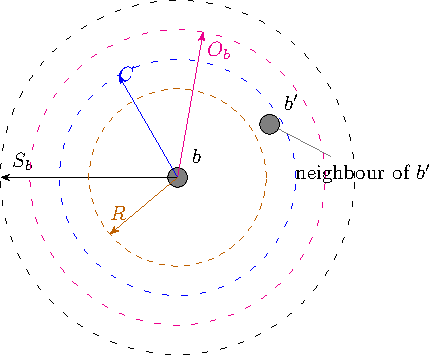
\includegraphics[width=0.8\linewidth]{figures/stableswarm}
	\caption[Agent Fields]{Agent Fields}
	\label{fig:stableswarm}
\end{figure}

\section{Related work}

As far back as 1987 swarm theory has adopted the use of field effects/potential fields to coordinate agents~\cite{REY:87} and this has continued since then in an attempt to improve the structure of a swarm, coordinate obstacles avoidance, and improve navigation~\cite{BAFVM:06,BAF:06,BFV:07,BM:09,eliot2018metric,VG:05,HC:09,SW:03,Son2017}. A prototype framework for self-healing swarms was developed by Dai et al., which considered how to manage agent failure in hostile environments \cite{DHMRZ:06}. This was similar to work by Vassev and Hinchey, who modelled swarm movement using the ASSL (Autonomic System Specification Language) \cite{VH:09}. This technique was employed by NASA (US National Aeronautics and Space Administration) for use in asteroid belt exploration as part of their ANTS (Autonomous Nano Technology Swarm) project. However, this work is focused towards failure of an agent's internal systems, rather than on the removal of anomalies in a swarm distribution. 

In the context of swarm structure maintenance, Roach et al. focussed on the effects of sensor failure, and the impact that has on agent distribution \cite{RMT:15}. Lee and Chong identified the issue of concave edges within swarms in an attempt to create regular lattice formations \cite{GN:08}, and the main focus of their work is the dynamic restructuring of inter-agent formations. Ismail and Timmis demonstrated the use of \textit{bio-inspired} healing using \textit{granuloma formation}, a biological method for encapsulating an antigen \cite{IT:10}. They have also considered the effect failed agents can have on a swarm when traversing a terrain~\cite{TIBW:16}. 

This void reduction effect through perimeter compression is an extension of the work presented by Eliot et al. \cite{eliot2019void}, Ismail and Timmis \cite{IT:10,TIBW:16}, and on the work of McLurkin and Demaine on the detection of perimeter types \cite{mclurkin2009}. However, perimeter type identification requires a communications infrastructure to allow the perimeter angle to be calculated. The technique employed in this paper does not explicitly require the identification of the perimeter type as it would limit the size of the swarm\cite{eliot2019void,GN:08} and is therefore a reduced algorithm to identify any perimeter.

\section{Basic swarming model}\label{basicModel}
In the Original work by Eliot et. al. the resultant vector of an agent was calculated using Equation~\ref{eq:resultantVector1a}. Where $k_c,k_r,k_d,k_o$ are weighting factors for the summed vectors associated with each interaction. i.e. $v_c$, $v_r$, $v_d$, $v_o$ for cohesion, repulsion, direction and object avoidance respectively. 

\begin{equation}\label{eq:resultantVector1a}
	v(b) = k_cv_c(b) + k_rv_r(b) + k_dv_d(b) + k_ov_o(b)
\end{equation}

In this paper we will only be considering the cohesion and repulsion components of the equation to create the new compression effect.

\subsection{Cohesion}\label{cohesion}
The cohesion component of an agent is calculated in a similar way to the repulsion in that it is dependent upon the proximity of neighbours. Where $n_c(b)$ is the set of neighbour agents for $b$ (Eq. \ref{eq:cohesion1}). The inclusion of an agent from a swarm ($S$) in by the agent's cohesion field ($C_b$).

\begin{equation}\label{eq:cohesion1}
n_c(b) = \{b' \in S~:~b' \neq b \land\magn{\vec{bb'}} \leq C_b\}
\end{equation}

The effect of an agent being within this set is that it will generate a vector that should `encourage' agents to maintain their proximity. i.e. generate a cohesive swarm. The general weighted ($k_c$) formula for agents to maintain their proximity is to direct their motion towards the central point of all neighbouring agents as shown in Equation~\ref{eq:cohesion2}. This formula includes the $k_c$ quotient that allows the cohesion effect to be `balanced' with respect to other vector influences as described in ~\cite{eliot2017methods,eliot2018metric,eliot2019void} 

\begin{equation}\label{eq:cohesion2}
v_c(b) = \frac{1}{\lvert n_c(b)\rvert} \sum_{b' \in n_c(b)}k_c\vec{bb'}
\end{equation}

\subsection{Repulsion}\label{repulsion:neighbours}
The repulsion component of an agent's movement is calculated from interaction with its neighbours $n_r(b)$ (Eq.~\ref{eq:repulsion1a}) in a swarm ($\mathcal{S}$) that are within the agent's ($b$) repulsion field ($R_b$).

\begin{equation}\label{eq:repulsion1a}
n_r(b) = \{b' \in \mathcal{S} : b \neq b' \land \lVert\vec{bb'}\rVert \leq R_b)\}
\end{equation}

The repulsion is then calculated as the average of all the vectors created by the agent ($b$) to the neighbours ($b'$) (Eg.~\ref{eq:repulsion2a}) and its proximity ($\lVert\vec{bb'}\rVert - R_b$).

\begin{equation}\label{eq:repulsion2a}
v_r(b) = \frac{1}{\lvert n_r(b)\rvert}\sum_{b' \in n_r(b)} \left(\lVert\vec{bb'}\rVert - R_b \, \right)\widehat{bb'}
\end{equation}

\section{Perimeter detection}\label{sec:perimeterDetection}
For perimeter compression to be applied to a swarm the perimeter needs to be detected. A perimeter can be defined as a continuous `surface' of agents that are not enclosed by other agents. These  agents may form an outer ({\color{green}green}) or inner ({\color{red}red}) boundary ~(Fig.~\ref{fig:innerOuterPerimeters}).

\begin{figure}[H]
	\begin{center}
		\includegraphics[width=5cm]{figures/PerimeterBots1}
	\end{center}
	\caption{{\color{green}Outer} and {\color{red}inner} swarm perimeters. \label{fig:innerOuterPerimeters}}
\end{figure}

The detection process is achieved using a cyclic analysis of the agents that surround an agent~(Fig.~\ref{fig:neighbours2}). Ghrist et al. discusses a similar technique using sweep angles~\cite{ghrist2008surrounding} as does McLurkin et al~\cite{mclurkin2009}. 

\begin{figure}[H]
	\centering
	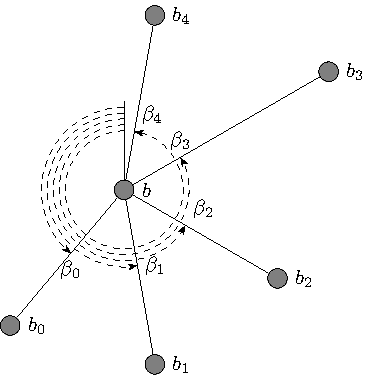
\includegraphics[width=0.8\linewidth]{figures/neighbours2}
	\caption[Agent neighbours]{Agent neighbours}
	\label{fig:neighbours2}
\end{figure}

The initial detection of the agents is based on the distance that each agent in the swarm is away from the current agent as described in Section~\ref{cohesion} and shown in Equation~\ref{eq:cohesion1}. The perimeter detection set is based on the azimuth angle ($\beta$) of each neighbour agent as shown in~Fig.~\ref{fig:neighbours2}.

The neighbour set $n_c(b)$ is then sorted in ascending order such that $\beta_0 < \beta_1 < \ldots < \beta_n$. Each consecutive pair of agents in the sequence now defines an \textit{edge} which has a length that can be calculated from their relative positions.

An agent is therefore on the perimeter of the swarm if it is not enclosed by the polygon defined in the sorted set $n_c(b)$. 

The polygon generated by $n_c(b)$ is considered to be `open' if two successive agents on the perimeter are separated by more than the size of the cohesion field ($C_b$).  

One further condition must be checked to detect a perimeter agent. When the polygon defined by $n_c(b)$ is closed it is possible that two or more neighbour agents are compressed to the point that they are with $C_b$ but are `behind' agent $b$. This condition can be detected based on any neighbour pair angle being greater than $\pi$. Figure~\ref{fig:neighbours3} shows this condition, assuming all the neighbour agent pairs are within range $C_b$. 

\begin{figure}[H]
	\centering
	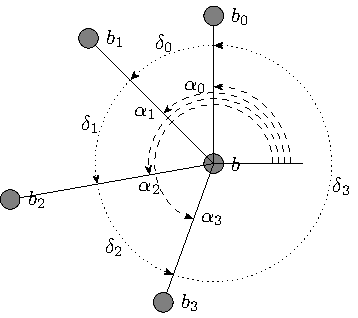
\includegraphics[width=0.8\linewidth]{figures/neighbours3}
	\caption[Agent neighbours]{Agent neighbour angles}
	\label{fig:neighbours3}
\end{figure}

\section{Perimeter compression model}
The new algorithm requires each individual agent to modify the movement vector generated based upon the perimeter status of the agent and each neighbour. The equation has been simplified (Eq.~\ref{eq:newModel2}) and the cohesion and repulsion weighting factors ($k_c,k_r$) have been transferred into the calculations. The additional weighting factors ($p_r,p_c$) are applied to specific agents within the cohesion and repulsion vector calculations.

% \begin{equation}\label{eq:newModel1}
% v(b) = v_c(b) + v_r(b) + v_d(b) + v_o(b)
% \end{equation}

As in the basic model (Section~\ref{basicModel}) the formula is simplified to only account for cohesion and repulsion~(Eq.~\ref{eq:newModel2}) although obstacle avoidance and direction can be added.

\begin{equation}\label{eq:newModel2}
v(b) = v_c(b) + v_r(b)
\end{equation}

The effect of introducing the additional weighting factors ($p_c$ and $p_r$) can be seen in \S~\ref{sec:ExperimentalResults} which demonstrates the additional internal disturbance of the swarm caused by the compression algorithm and the removal of internal swarm voids. 

Figure~\ref{fig:voidRemoval} shows how the compression effect can remove a void from a swarm by surround an obstacle in a similar manner to the method described by Eliot et al. in~\cite{eliot2019void}.

\begin{figure}
\centering
\begin{subfigure}{0.4\textwidth}
	\centering	
	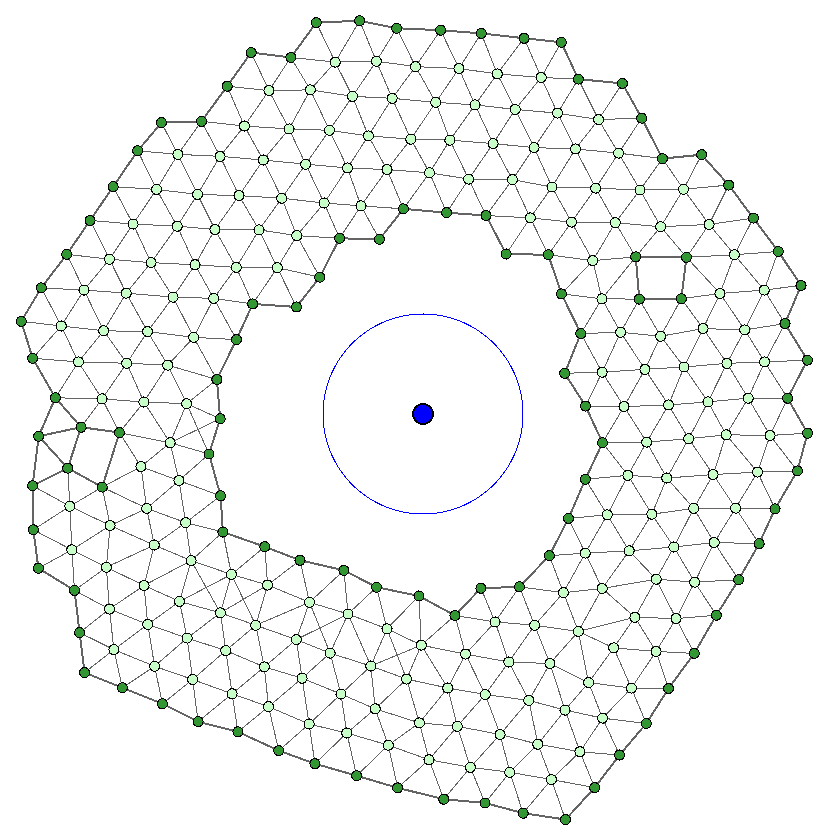
\includegraphics[width=1.0\linewidth]{figures/voidRemoval1}
	\caption[Void removal start]{Void removal start}
	\label{fig:voidRemovalStart}
\end{subfigure}
\begin{subfigure}{0.4\textwidth}
	\centering
	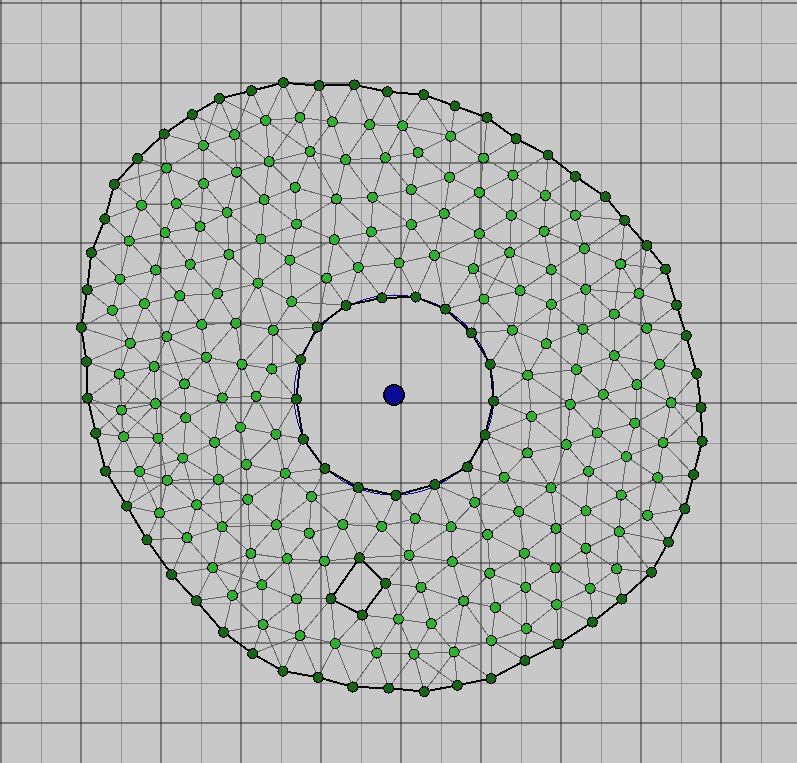
\includegraphics[width=1.0\linewidth]{figures/voidRemoval2}
	\caption[Void removal finish]{Void removal finish}
	\label{fig:voidRemovalFinish}
\end{subfigure}
\caption{Void removal through perimeter compression}
\label{fig:voidRemoval}
\end{figure}

\subsection{Modified cohesion model}
The cohesion component of the compression effect ($p_c$) is applied when an agent ($b$) and its neighbour ($b'$) are both perimeter-based. If the agents are not both perimeter-based then the agents cohesion vector is scaled by $k_c$ (Eq.~\ref{eq:cohesion4}). The effect of the additional cohesion-compression weighting is to increases the size of the effective, generated cohesion-vector (\textbf{ef}fective \emph{c}ohesion) $\mathsf{efc}(b,b')$ (Eq.~\ref{eq:cohesion3}) which causes the agent to have a tendency to move towards that neighbour. 

\begin{equation}\label{eq:cohesion3}
v_c(b) = \frac{1}{\lvert n_c(b)\rvert} \sum_{b' \in n_c(b)}\mathsf{ekc}(b, b')\, \vec{bb'}
\end{equation}

\small
\begin{equation}\label{eq:cohesion4}
\mathsf{ekc}(b, b') = \mathsf{if} \; \mathsf{per}(b) \; \mathsf{and} \; \mathsf{per}(b') \; \mathsf{then} \; \mathrm{p}_ck_c \; \mathsf{else} \; k_c
\end{equation}
\normalsize

\subsection{Modified repulsion model}\label{repulsion:compression}
The repulsion compression component of the perimeter is applied by adjusted the \textbf{e}ffective \textbf{r}ange \textbf{f}ield ($\mathsf{erf}(b,b')$) if the agents are both perimeter-based. Equation~\ref{eq:repulsion2} shows the new formula to calculate the adjusted repulsion. As the agent's repulsion field is always within the cohesion field (Eq.~\ref{eq:cohesion1}), the repulsion neighbours can also be defined as a subset of the cohesion neighbours $n_c(b)$~(Eq.~\ref{eq:repulsion3}).\\

\begin{equation}\label{eq:repulsion1}
n_r(b) = \{b' \in \mathcal{S} : b \neq b' \land \lVert\vec{bb'}\rVert \leq \mathsf{erf}(b,b')\}
\end{equation}

% \small
% \begin{equation}\label{eq:repulsion2}
% \mathsf{erf}(b, b') = \mathsf{if} \;
% \mathsf{per}(b) \; \mathsf{and} \; \mathsf{per}(b') \; \mathsf{then} \;
% p_rR_b \; \mathsf{else} \; R_b
% \end{equation}
\normalsize

\begin{equation}\label{eq:repulsion3}
n_r(b) = \{b' \in n_c(b)~:~\magn{\vec{bb'}} <= \mathsf{erf}(b,b')\}
\end{equation}

An agent is identified as a perimeter agent using the technique described in \S~\ref{sec:perimeterDetection} and shown by Eliot et.al. in \cite{eliot2019void} which uses a cyclic-check of neighbour agent angles to identify `gaps' in the neighbours.

If the condition of both agents being a perimeter is met ($\mathsf{per}(b) \; \mathsf{and} \; \mathsf{per}(b')$) the repulsion field distance is multiplied by the compression factor ($p_r$) and the new field effect is used to generate a resultant-repulsion-vector (Eq.~\ref{eq:repulsion5}). 

The effect of Equation \ref{eq:repulsion4} will be to reduce the repulsion of inter-perimeter-based agents allowing them to be closer together before a reduced repulsion-vector is applied. 

\important{The repulsion-vector that is generated is based upon $p_rR_b$, the reduced repulsion field, and not the full $R_b$ field. This is to scale the resultant-repulsion-vector as well as reducing the repulsion field.}
\small
\begin{equation}\label{eq:repulsion4}
v_r(b) = \frac{1}{\lvert n_r(b)\rvert}\sum_{b' \in n_r(b)} k_r\left(\lVert\vec{bb'}\rVert - \mathsf{erf}(b,b') \, \right)\widehat{bb'}
\end{equation}
\normalsize
\small
\begin{equation}\label{eq:repulsion5}
\mathsf{erf}(b, b') = \mathsf{if} \;
\mathsf{per}(b) \; \mathsf{and} \; \mathsf{per}(b') \; \mathsf{then} \;
p_rR_b \; \mathsf{else} \; R_b
\end{equation}
\normalsize

\section{Experimental results\label{sec:ExperimentalResults}}
\subsection{Baseline}
For all the experiments the parameters used to create the basic swarming effect are shown in Table~\ref{tab:swarmingEffect}. Where $C_b$ is the cohesion field, $k_c$ is the cohesion weighting, $R_b$ is the repulsion field, $k_r$ is the repulsion weighting. The swarm consists of 200 agents which are distributed with a void at the centre. These initial parameters create a hexagonal-based distribution of agents that stabilise as shown in Figure~\ref{fig:baselineSwarm}. This basic swarm is used as the initial state for all the experiments. 
 \begin{table}[h]
	\centering
	\tiny
	\begin{tabular}{|c|r|}
		\hline
		\rowcolor[HTML]{000000} 
		{\color[HTML]{FFFFFF} Swarming Variable} & {\color[HTML]{FFFFFF} Value} \\ \hline
		$C_b$ & \texttt{3.00} \\ \hline
		$k_c$ & \texttt{0.15}  \\ \hline
		$R_b$ & \texttt{2.00} \\ \hline
		$k_r$ & \texttt{50.00} \\ \hline
		$k_g$ & \texttt{25.00} \\ \hline
	\end{tabular}
  	\caption{Swarming effect parameters}
  	\label{tab:swarmingEffect}
\end{table}

\begin{figure}[H]
	\begin{center}
		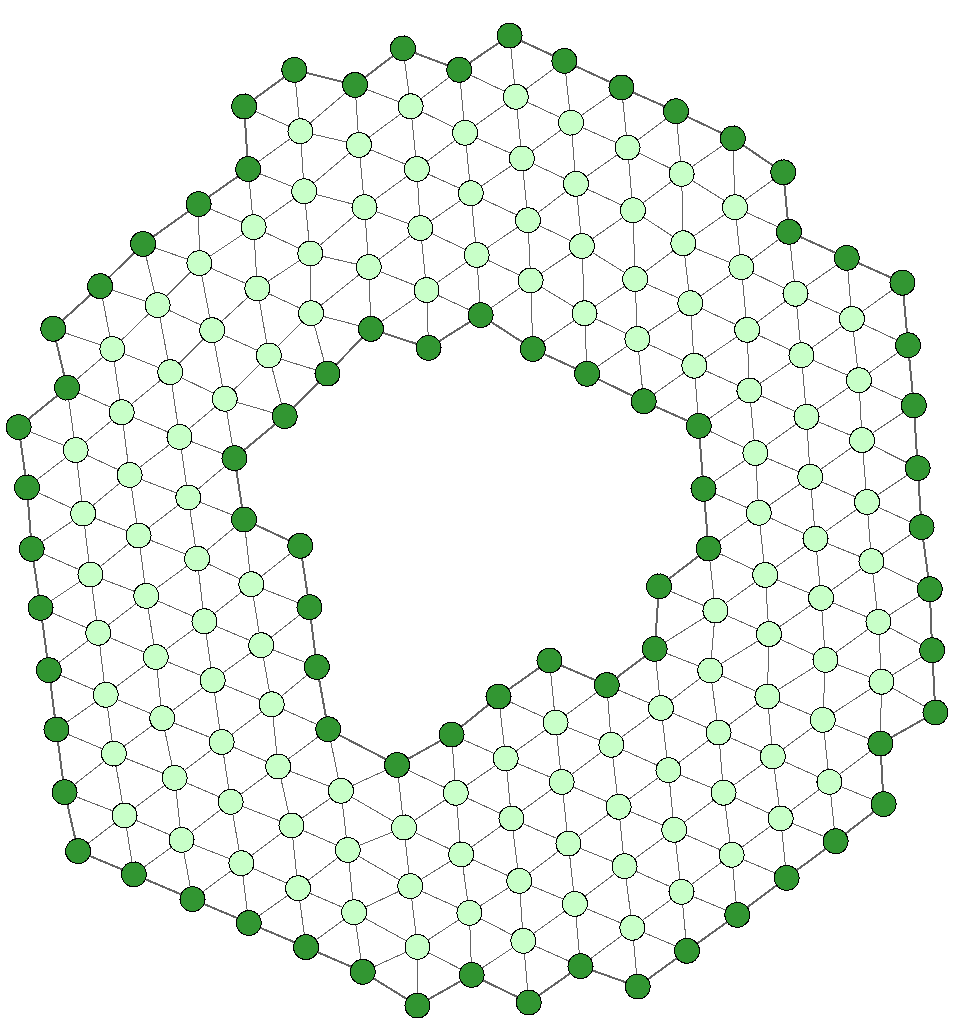
\includegraphics[width=5cm]{figures/exp1Start}
	\end{center}
	\caption{Baseline swarm in stabilised configuration. \label{fig:baselineSwarm}}
\end{figure}

When the simulation is ran with no compression the resultant magnitudes generated are shown in Table~\ref{fig:baselineSwarmMagnitude}. These states are used as the baseline for the experiments to measure the effects of the compression algorithm and compare the new algorithm to the existing void reduction algorithm discussed by Eliot et al. in~\cite{eliot2018metric}.

\begin{figure}[H]
	\begin{center}
		\includegraphics[width=8cm]{figures/interagentMagnitudeBaseline}
	\end{center}
	\caption{Baseline swarm in stabilised configuration. \label{fig:baselineSwarmMagnitude}}
\end{figure}

\subsection{Compression Effects\label{sec:CompressionEffect}}

The compression effect parameters are shown in table~\ref{tab:compressionEffect}
\begin{table}[h]
	\centering
	\tiny
	\begin{tabular}{|c|r|r|r|r|r|r|}
		\hline
		\rowcolor[HTML]{000000} 
		{\color[HTML]{FFFFFF} Comp.} & {\color[HTML]{FFFFFF} 1} & {\color[HTML]{FFFFFF} 2} & {\color[HTML]{FFFFFF} 3} & {\color[HTML]{FFFFFF} 4} & {\color[HTML]{FFFFFF} 5} & {\color[HTML]{FFFFFF} 6}\\ \hline
		$p_r$ & \texttt{0.10} & \texttt{0.15} & \texttt{0.20} & \texttt{0.25} & \texttt{0.30} & \texttt{0.35} \\ \hline
		$p_c$ & \texttt{20.00}  & \texttt{30.00} & \texttt{40.00} & \texttt{50.00} & \texttt{60.00} & \texttt{70.00}\\ \hline
	\end{tabular}
	\caption{Compression effect parameters}
	\label{tab:compressionEffect}
\end{table}

\begin{table}[h]
	\centering
	\tiny
\begin{tabular}{ | >{\columncolor[HTML]{000000}}l | l | l | l | l | l | }
	\hline
	\rowcolor[HTML]{000000} 
	{\color[HTML]{FFFFFF} Pr/Pc} & {\color[HTML]{FFFFFF}10} & {\color[HTML]{FFFFFF}20} & {\color[HTML]{FFFFFF}30} & {\color[HTML]{FFFFFF}40} & {\color[HTML]{FFFFFF}50} \\ \hline
	    {\color[HTML]{FFFFFF}0.1} & 0.1/10 & 0.1/20 & 0.1/30 & 0.1/40 & 0.1/50  \\ \hline
		{\color[HTML]{FFFFFF}0.2} & 0.2/10 & 0.2/20 & 0.2/30 & 0.2/40 & 0.2/50  \\ \hline
		{\color[HTML]{FFFFFF}0.3} & 0.3/10 & 0.3/20 & 0.3/30 & 0.3/40 & 0.3/50  \\ \hline
		{\color[HTML]{FFFFFF}0.4} & 0.4/10 & 0.4/20 & 0.4/30 & 0.4/40 & 0.4/50  \\ \hline
		{\color[HTML]{FFFFFF}0.5} & 0.5/10 & 0.5/20 & 0.5/30 & 0.5/40 & 0.5/50  \\ \hline
		{\color[HTML]{FFFFFF}0.6} & 0.6/10 & 0.6/20 & 0.6/30 & 0.6/40 & 0.6/50  \\ \hline
		{\color[HTML]{FFFFFF}0.7} & 0.7/10 & 0.7/20 & 0.7/30 & 0.7/40 & 0.7/50  \\ \hline
		{\color[HTML]{FFFFFF}0.8} & 0.8/10 & 0.8/20 & 0.8/30 & 0.8/40 & 0.8/50  \\ \hline
		{\color[HTML]{FFFFFF}0.9} & 0.9/10 & 0.9/20 & 0.9/30 & 0.9/40 & 0.9/50  \\ \hline
	\end{tabular}
	\caption{Experiment parameters 1}
	\label{tab:compressionExperimentEffect1}
\end{table}

\begin{table}[h]
	\centering
	\tiny
\begin{tabular}{ | >{\columncolor[HTML]{000000}}l | l | l | l | l | l | }
	\hline
	\rowcolor[HTML]{000000} 
	{\color[HTML]{FFFFFF} Pr/Pc} & {\color[HTML]{FFFFFF}60} & {\color[HTML]{FFFFFF}70} & {\color[HTML]{FFFFFF}80} & {\color[HTML]{FFFFFF}90} & {\color[HTML]{FFFFFF}100}   \\ \hline
		{\color[HTML]{FFFFFF}0.1} & 0.1/60 & 0.1/70 & 0.1/80 & 0.1/90 & 0.1/100 \\ \hline
		{\color[HTML]{FFFFFF}0.2} & 0.2/60 & 0.2/70 & 0.2/80 & 0.2/90 & 0.2/100 \\ \hline
		{\color[HTML]{FFFFFF}0.3} & 0.3/60 & 0.3/70 & 0.3/80 & 0.3/90 & 0.3/100 \\ \hline
		{\color[HTML]{FFFFFF}0.4} & 0.4/60 & 0.4/70 & 0.4/80 & 0.4/90 & 0.4/100 \\ \hline
		{\color[HTML]{FFFFFF}0.5} & 0.5/60 & 0.5/70 & 0.5/80 & 0.5/90 & 0.5/100 \\ \hline
		{\color[HTML]{FFFFFF}0.6} & 0.6/60 & 0.6/70 & 0.6/80 & 0.6/90 & 0.6/100 \\ \hline
		{\color[HTML]{FFFFFF}0.7} & 0.7/60 & 0.7/70 & 0.7/80 & 0.7/90 & 0.7/100 \\ \hline
		{\color[HTML]{FFFFFF}0.8} & 0.8/60 & 0.8/70 & 0.8/80 & 0.8/90 & 0.8/100 \\ \hline
		{\color[HTML]{FFFFFF}0.9} & 0.9/60 & 0.9/70 & 0.9/80 & 0.9/90 & 0.9/100 \\ \hline
	\end{tabular}
	\caption{Experiment parameters 2}
	\label{tab:compressionExperimentEffect2}
\end{table}

\begin{figure}[H]
	\begin{center}
		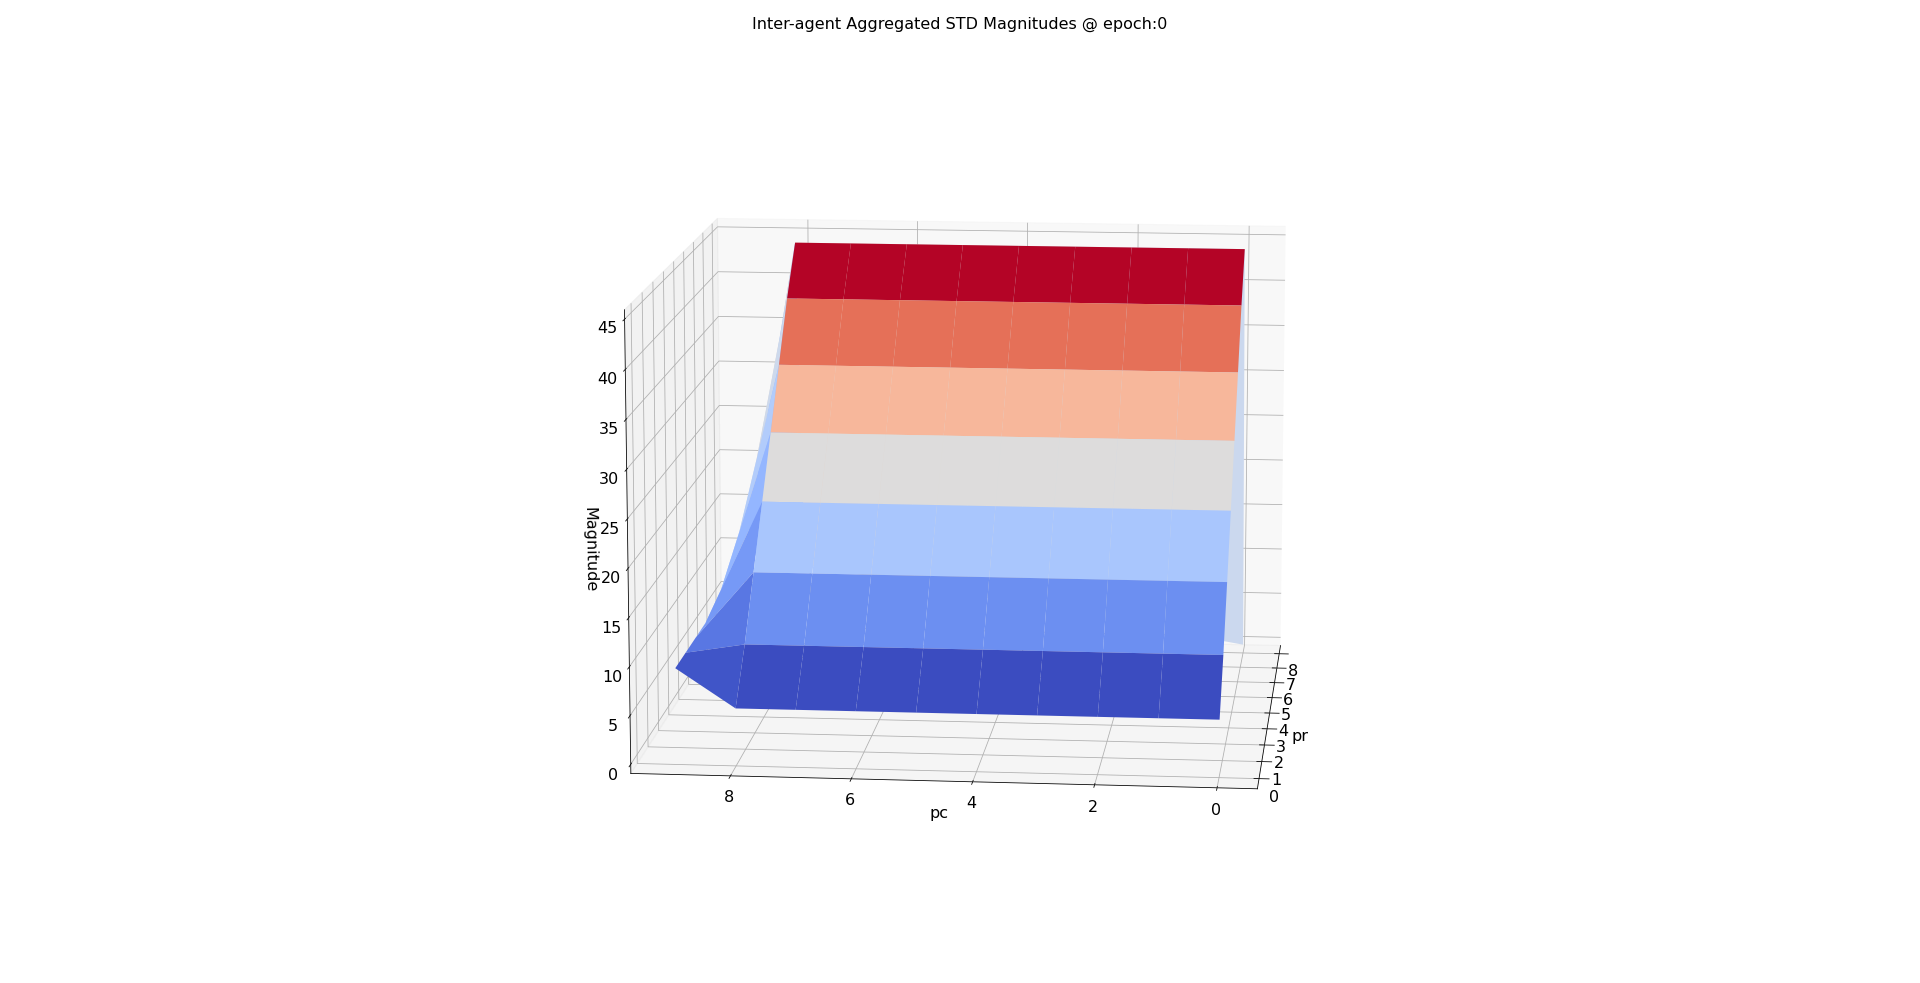
\includegraphics[width=8cm]{figures/Experiment1}
	\end{center}
	\caption{Experiment Start \label{fig:experiment1}}
\end{figure}

\begin{figure}[H]
	\begin{center}
		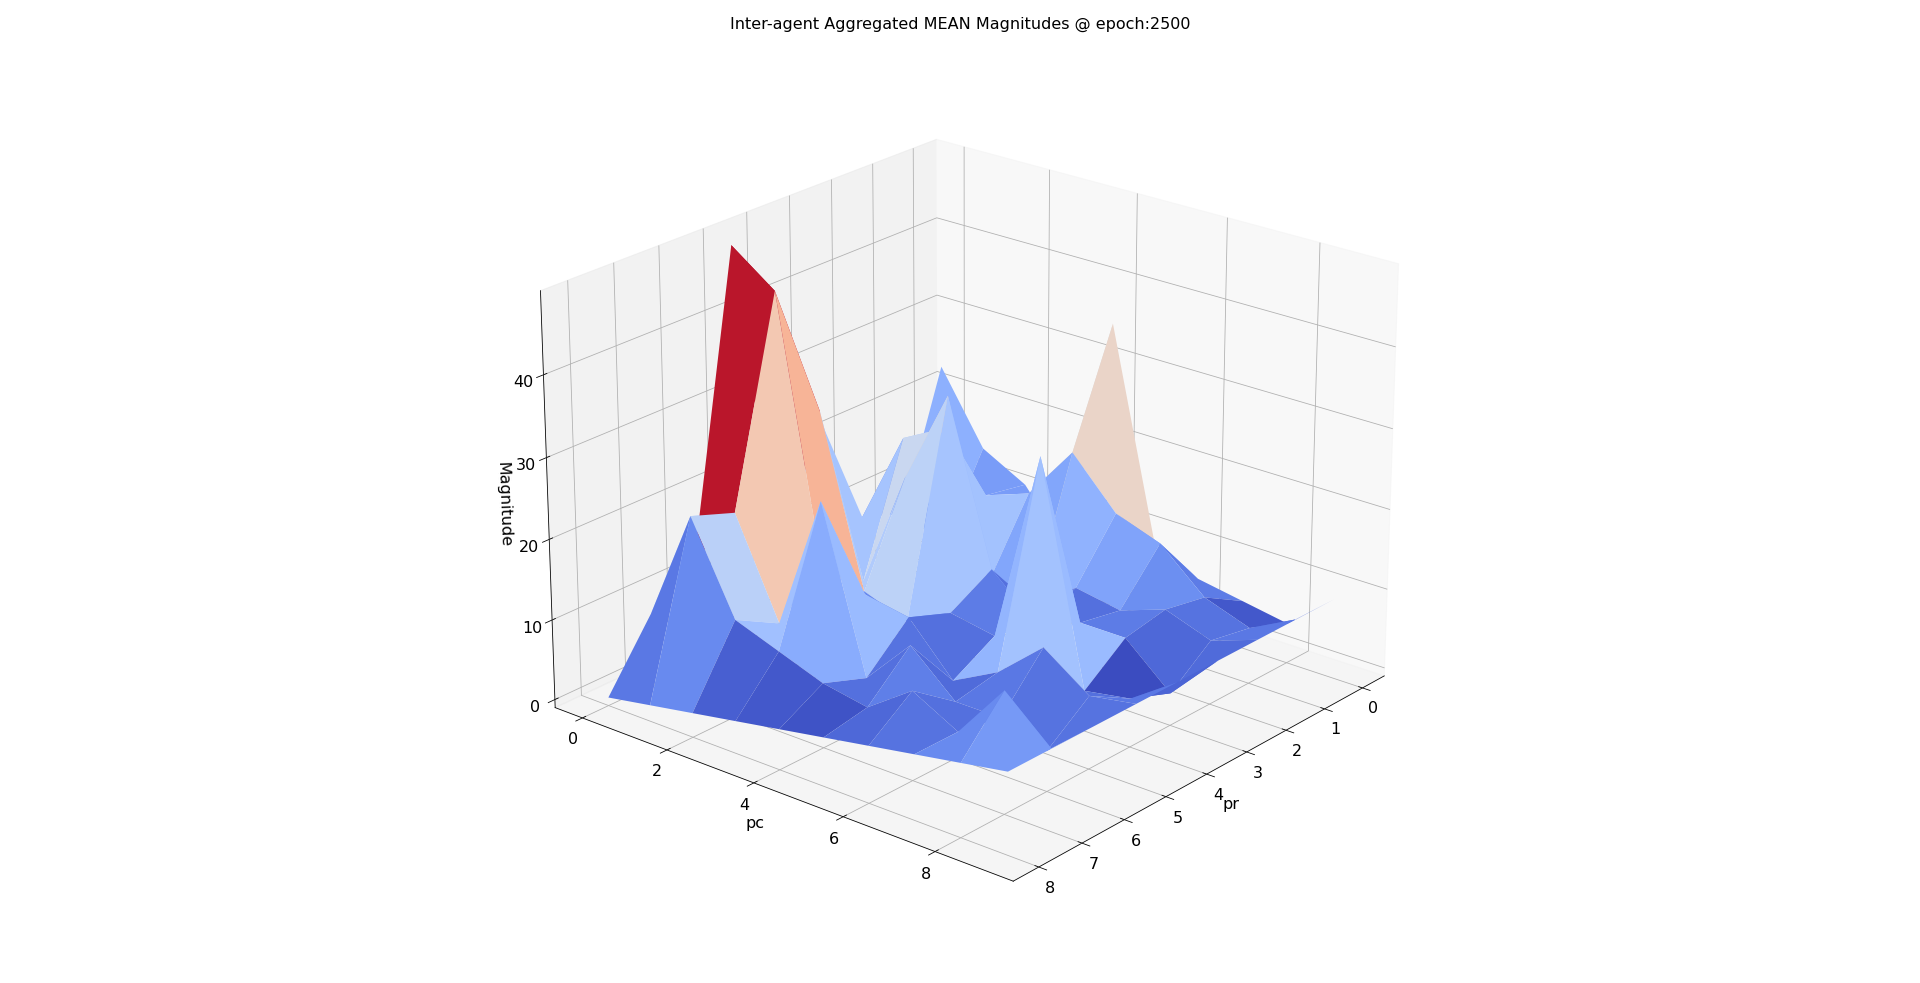
\includegraphics[width=8cm]{figures/Experiment2}
	\end{center}
	\caption{Experiment Middle \label{fig:experiment2}}
\end{figure}

\begin{figure}[H]
	\begin{center}
		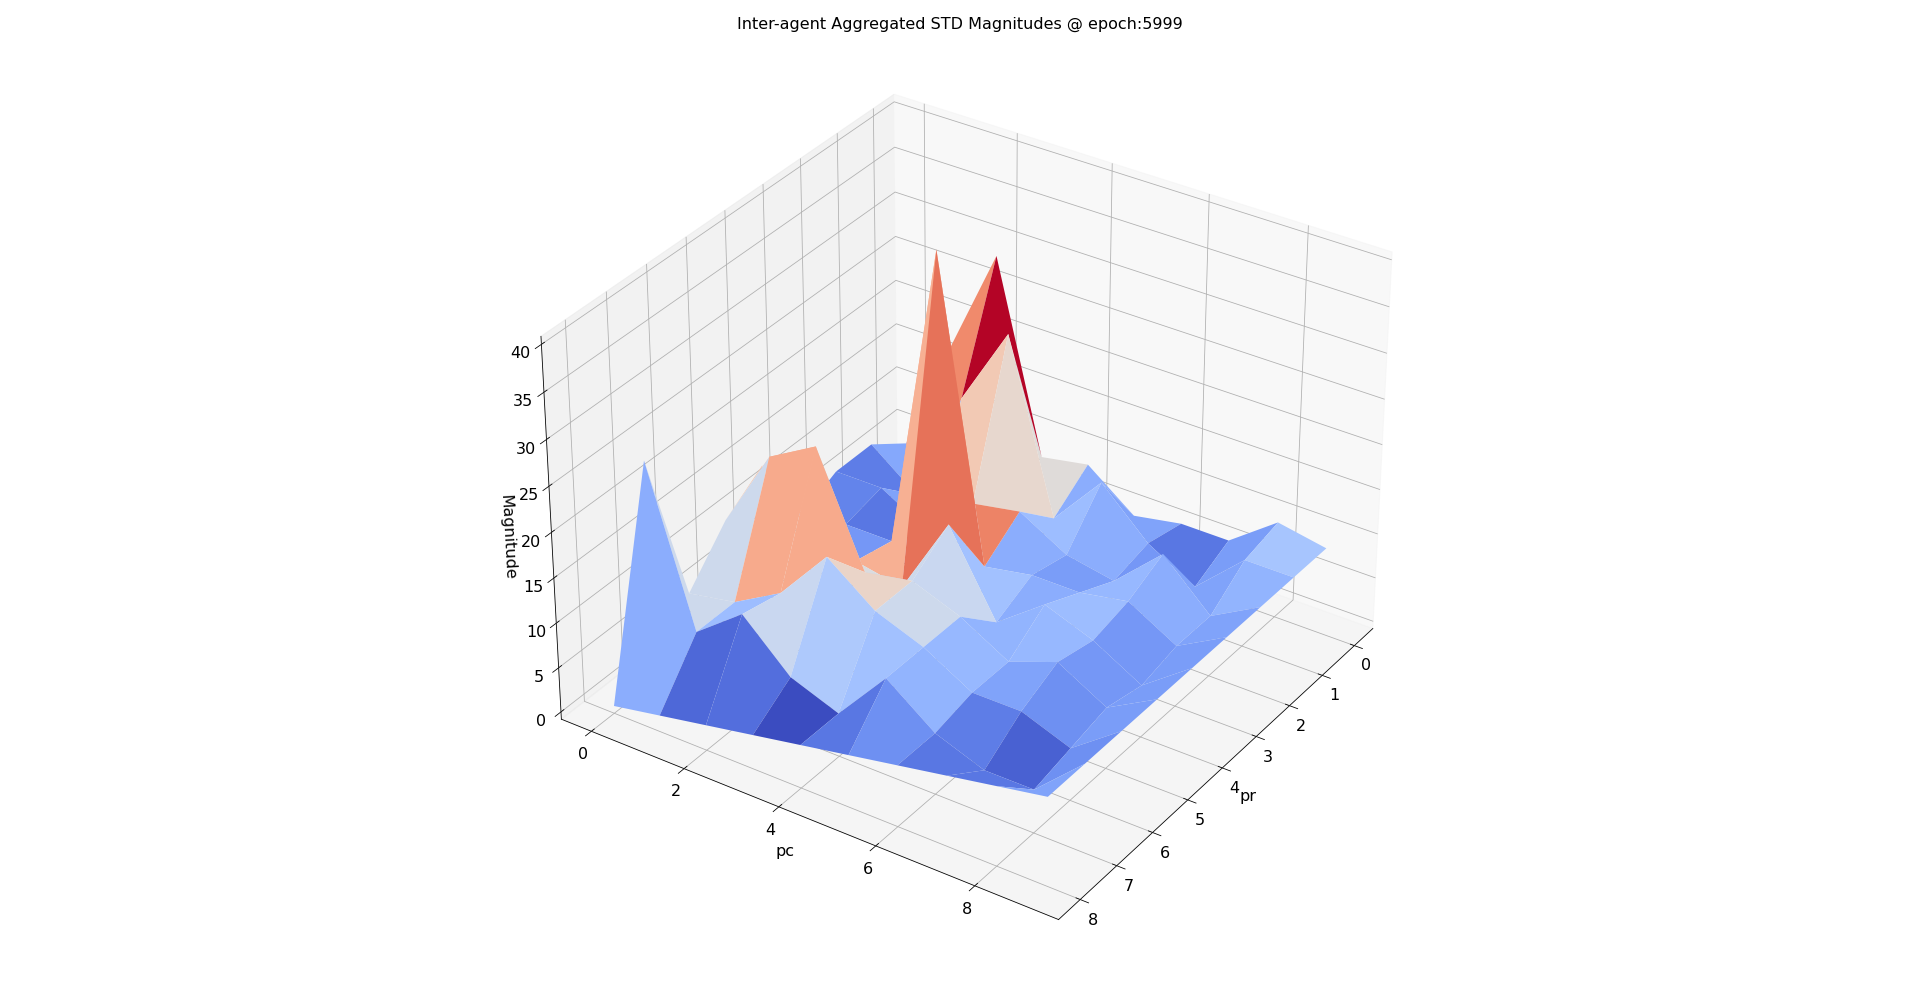
\includegraphics[width=8cm]{figures/Experiment3}
	\end{center}
	\caption{Experiment End \label{fig:experiment3}}
\end{figure}

The first area of comparison is the effect of the algorithms on the number of perimeter agents. The baseline swarm's agents oscillates but remain in a relatively stable state with a constant number of perimeter agents and the internal anomaly persists~(Fig.~\ref{fig:baselineSwarm}). The maximum and minimum number of perimeter agents is shown in table~\ref{tab:perimeterLimits}. 

\begin{figure}[H]
	\begin{center}
		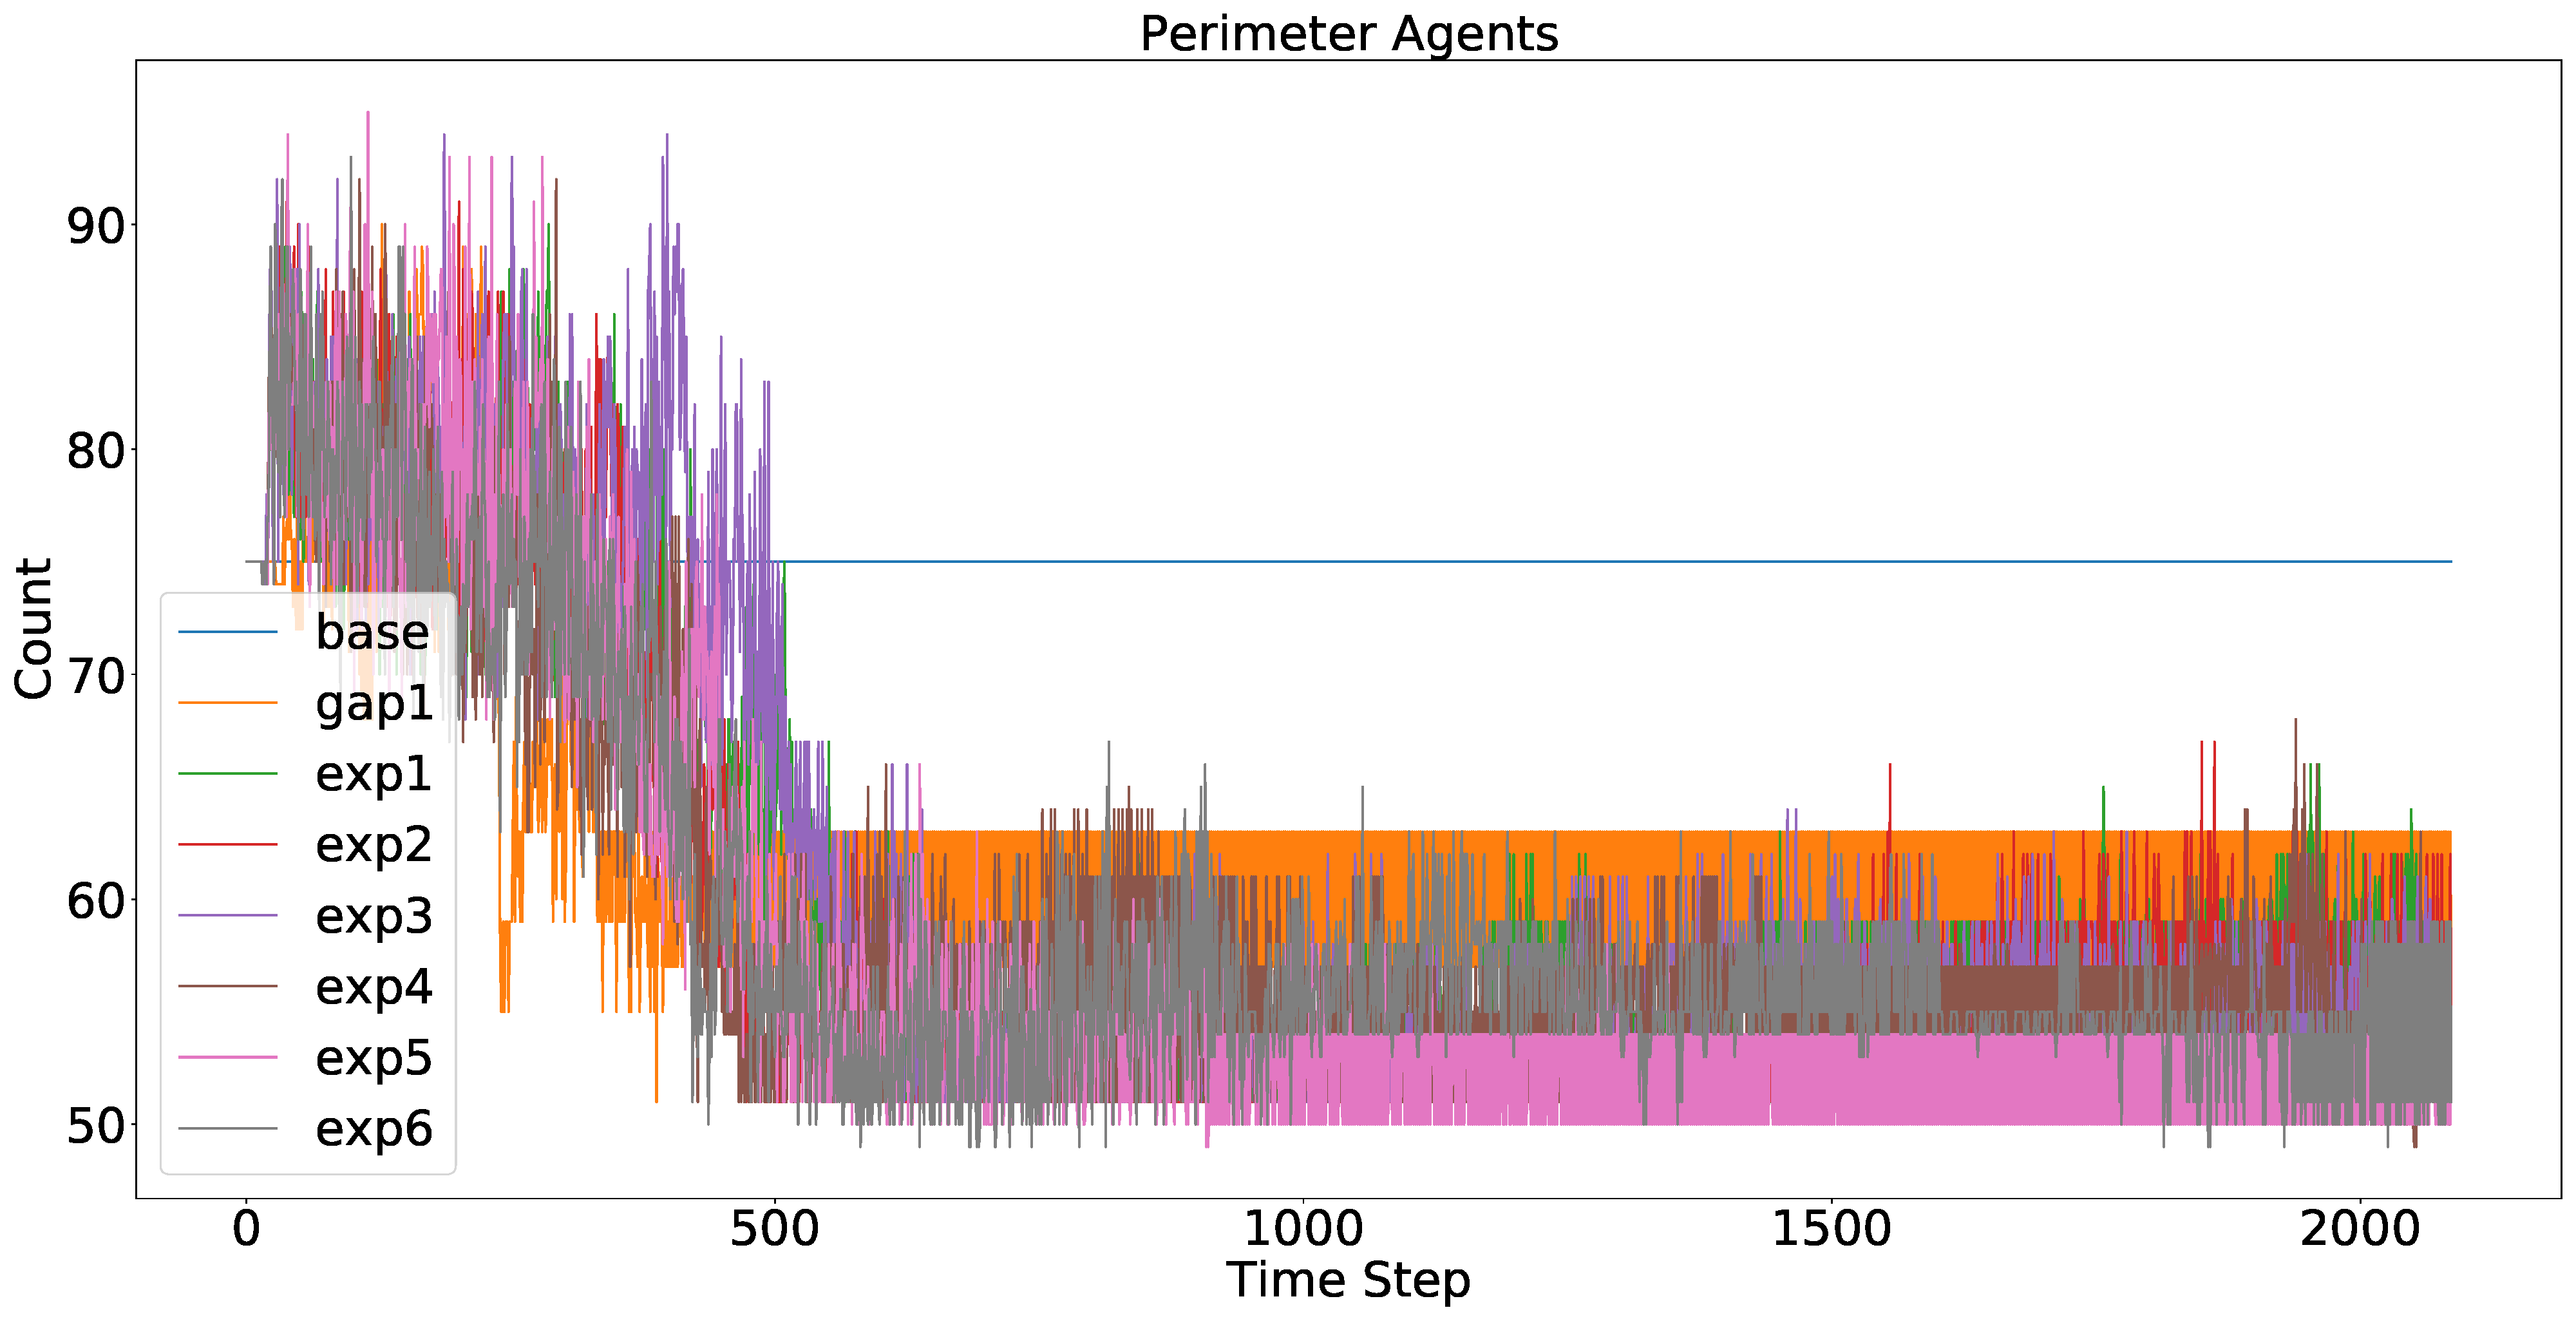
\includegraphics[width=8cm]{figures/PerimeterCount}
	\end{center}
	\caption{Perimeter Count of baseline, gap reduction and perimeter compression. \label{fig:perimeterCount}}
\end{figure}

\begin{table}[h]
	\centering
	\tiny
	\begin{tabular}{|c|c|r|r|r|r|r|r|r|}
		\hline
		\rowcolor[HTML]{000000} 
		{\color[HTML]{FFFFFF} Comp.} &{\color[HTML]{FFFFFF} Base} & {\color[HTML]{FFFFFF} Void} & {\color[HTML]{FFFFFF} 1} & {\color[HTML]{FFFFFF} 2} & {\color[HTML]{FFFFFF} 3} & {\color[HTML]{FFFFFF} 4} & {\color[HTML]{FFFFFF} 5} & {\color[HTML]{FFFFFF} 6}\\ \hline
		Max & \texttt{75} & \texttt{90} &\texttt{90} & \texttt{90} & \texttt{94} & \texttt{92} & \texttt{95} & \texttt{93} \\ \hline
		Min & \texttt{75} & \texttt{51} &\texttt{51}  & \texttt{51} & \texttt{51} & \texttt{49} & \texttt{49} & \texttt{49}\\ \hline
		Mean & \texttt{75} & \texttt{62} &\texttt{59}  & \texttt{58} & \texttt{60} & \texttt{59} & \texttt{57} & \texttt{59}\\ \hline
		Std & \texttt{0} & \texttt{6} &\texttt{9}  & \texttt{10} & \texttt{10} & \texttt{8} & \texttt{10} & \texttt{8}\\ \hline
	\end{tabular}
	\caption{Perimeter agents}
	\label{tab:perimeterLimits}
\end{table}

\begin{figure}[H]
	\begin{center}
		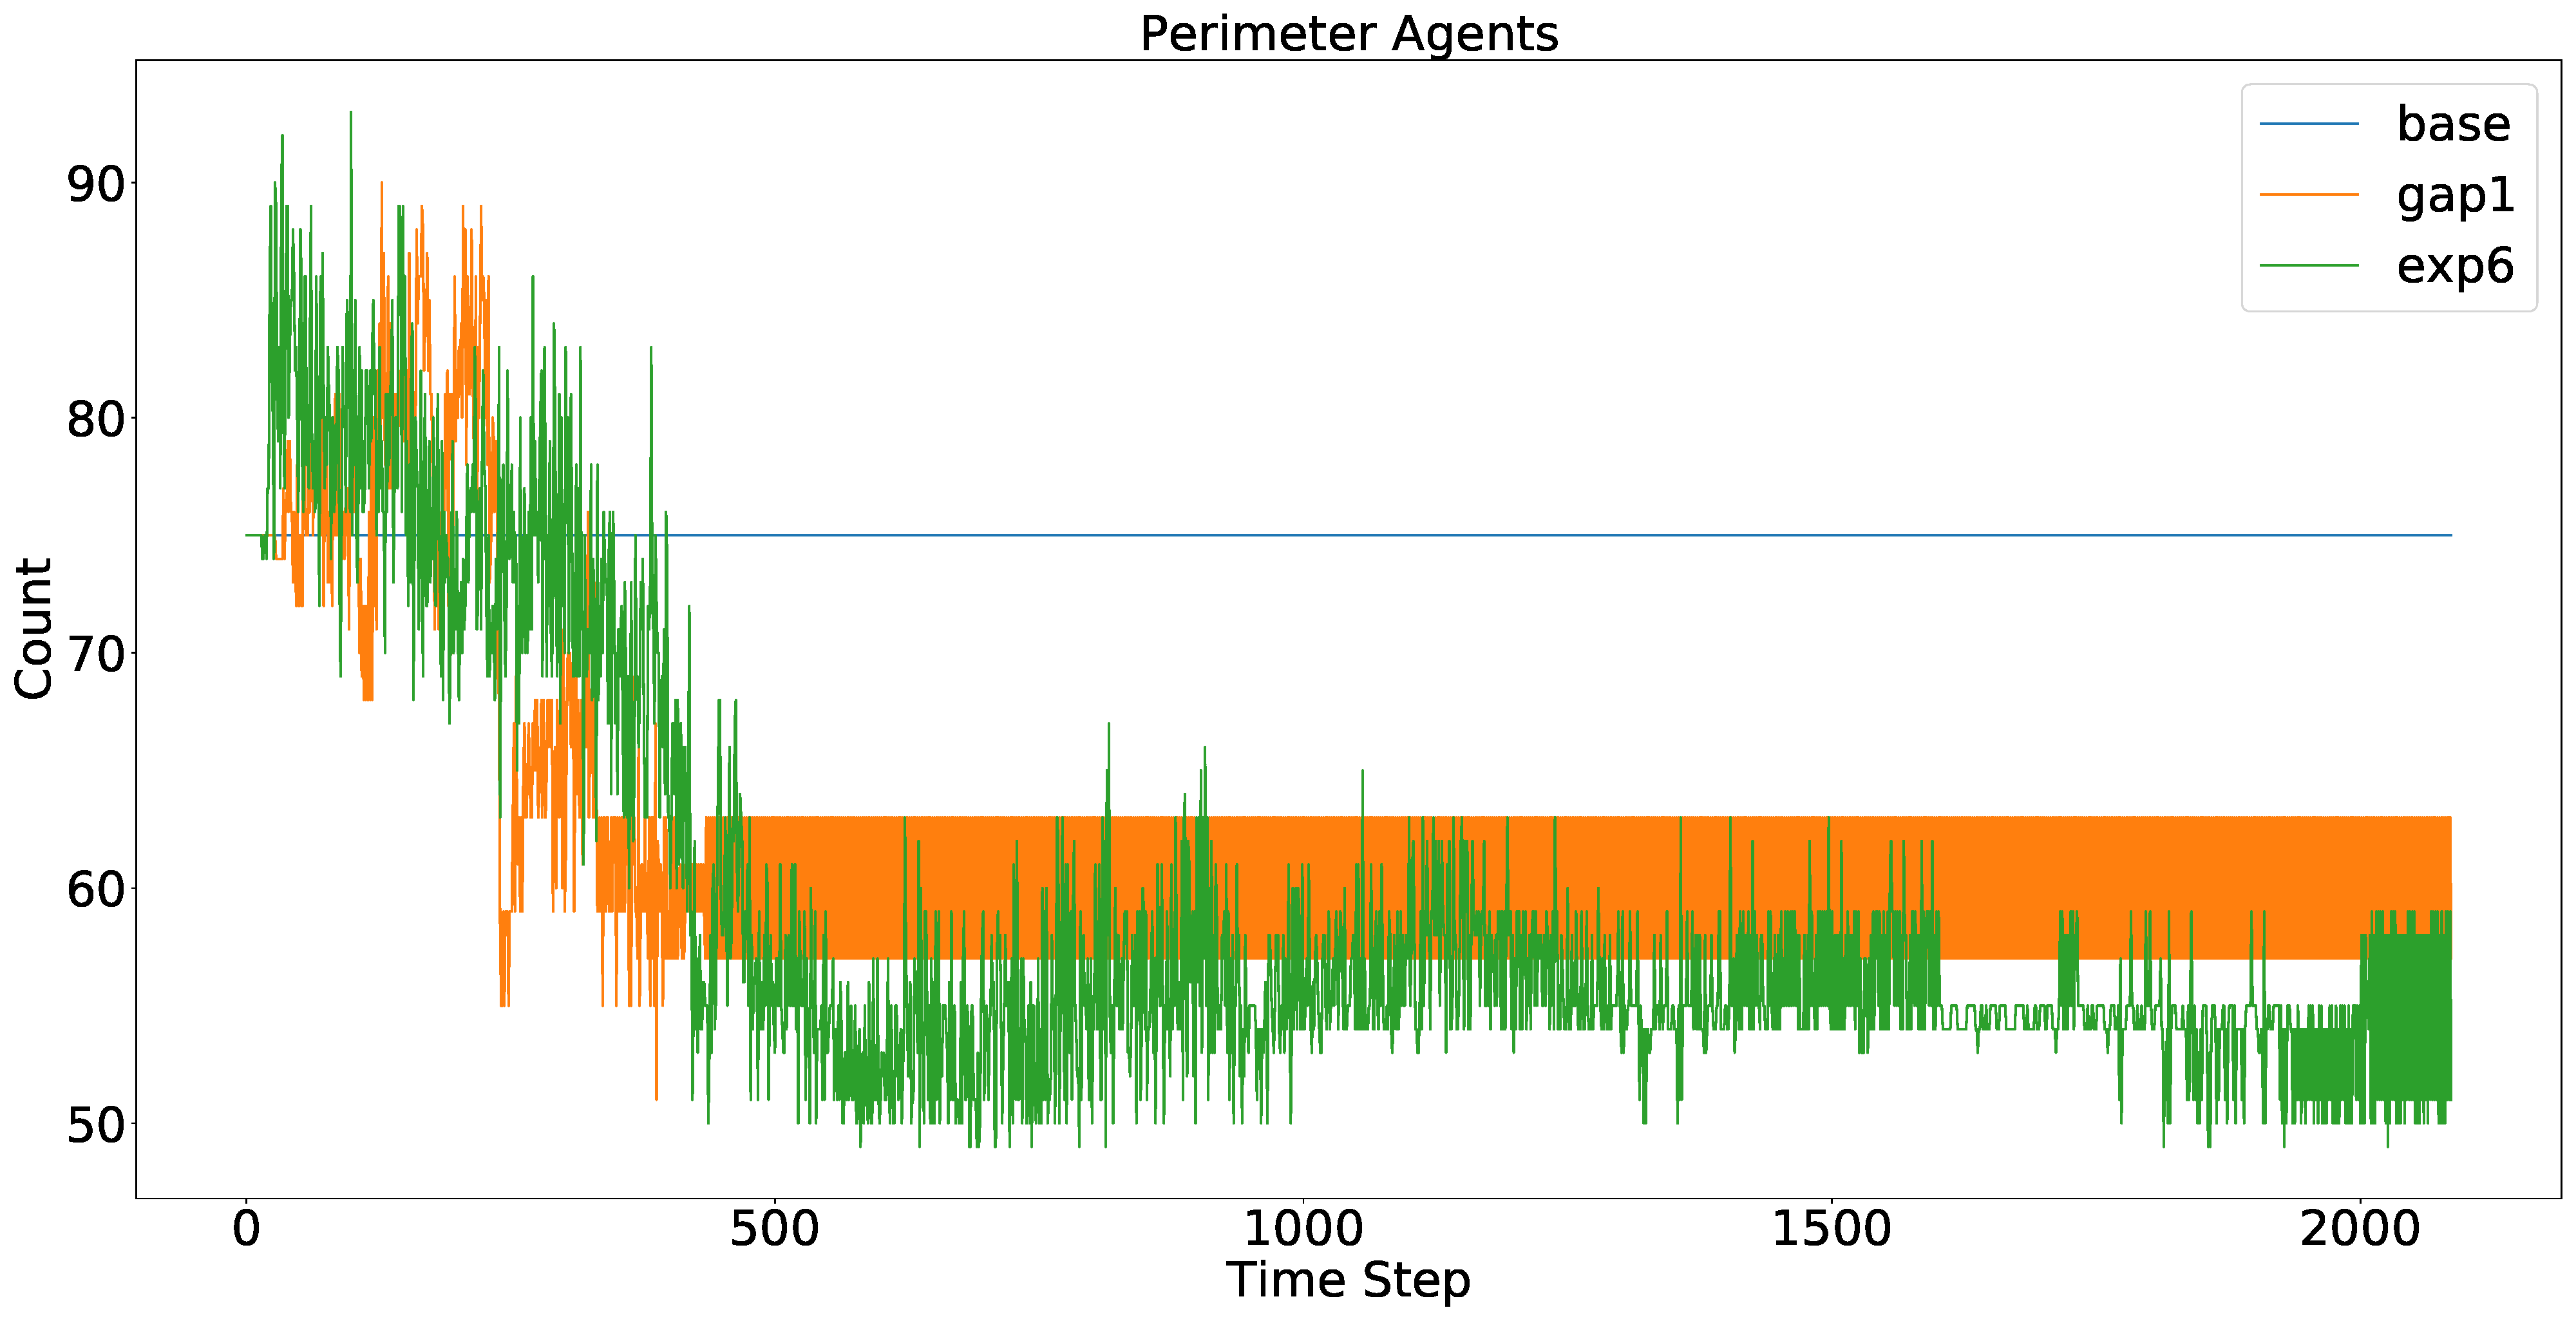
\includegraphics[width=8cm]{figures/PerimeterCount2}
	\end{center}
	\caption{Perimeter Count of baseline, gap reduction and Experiment 6. \label{fig:perimeterCount2}}
\end{figure}

\begin{figure}[H]
	\begin{center}
		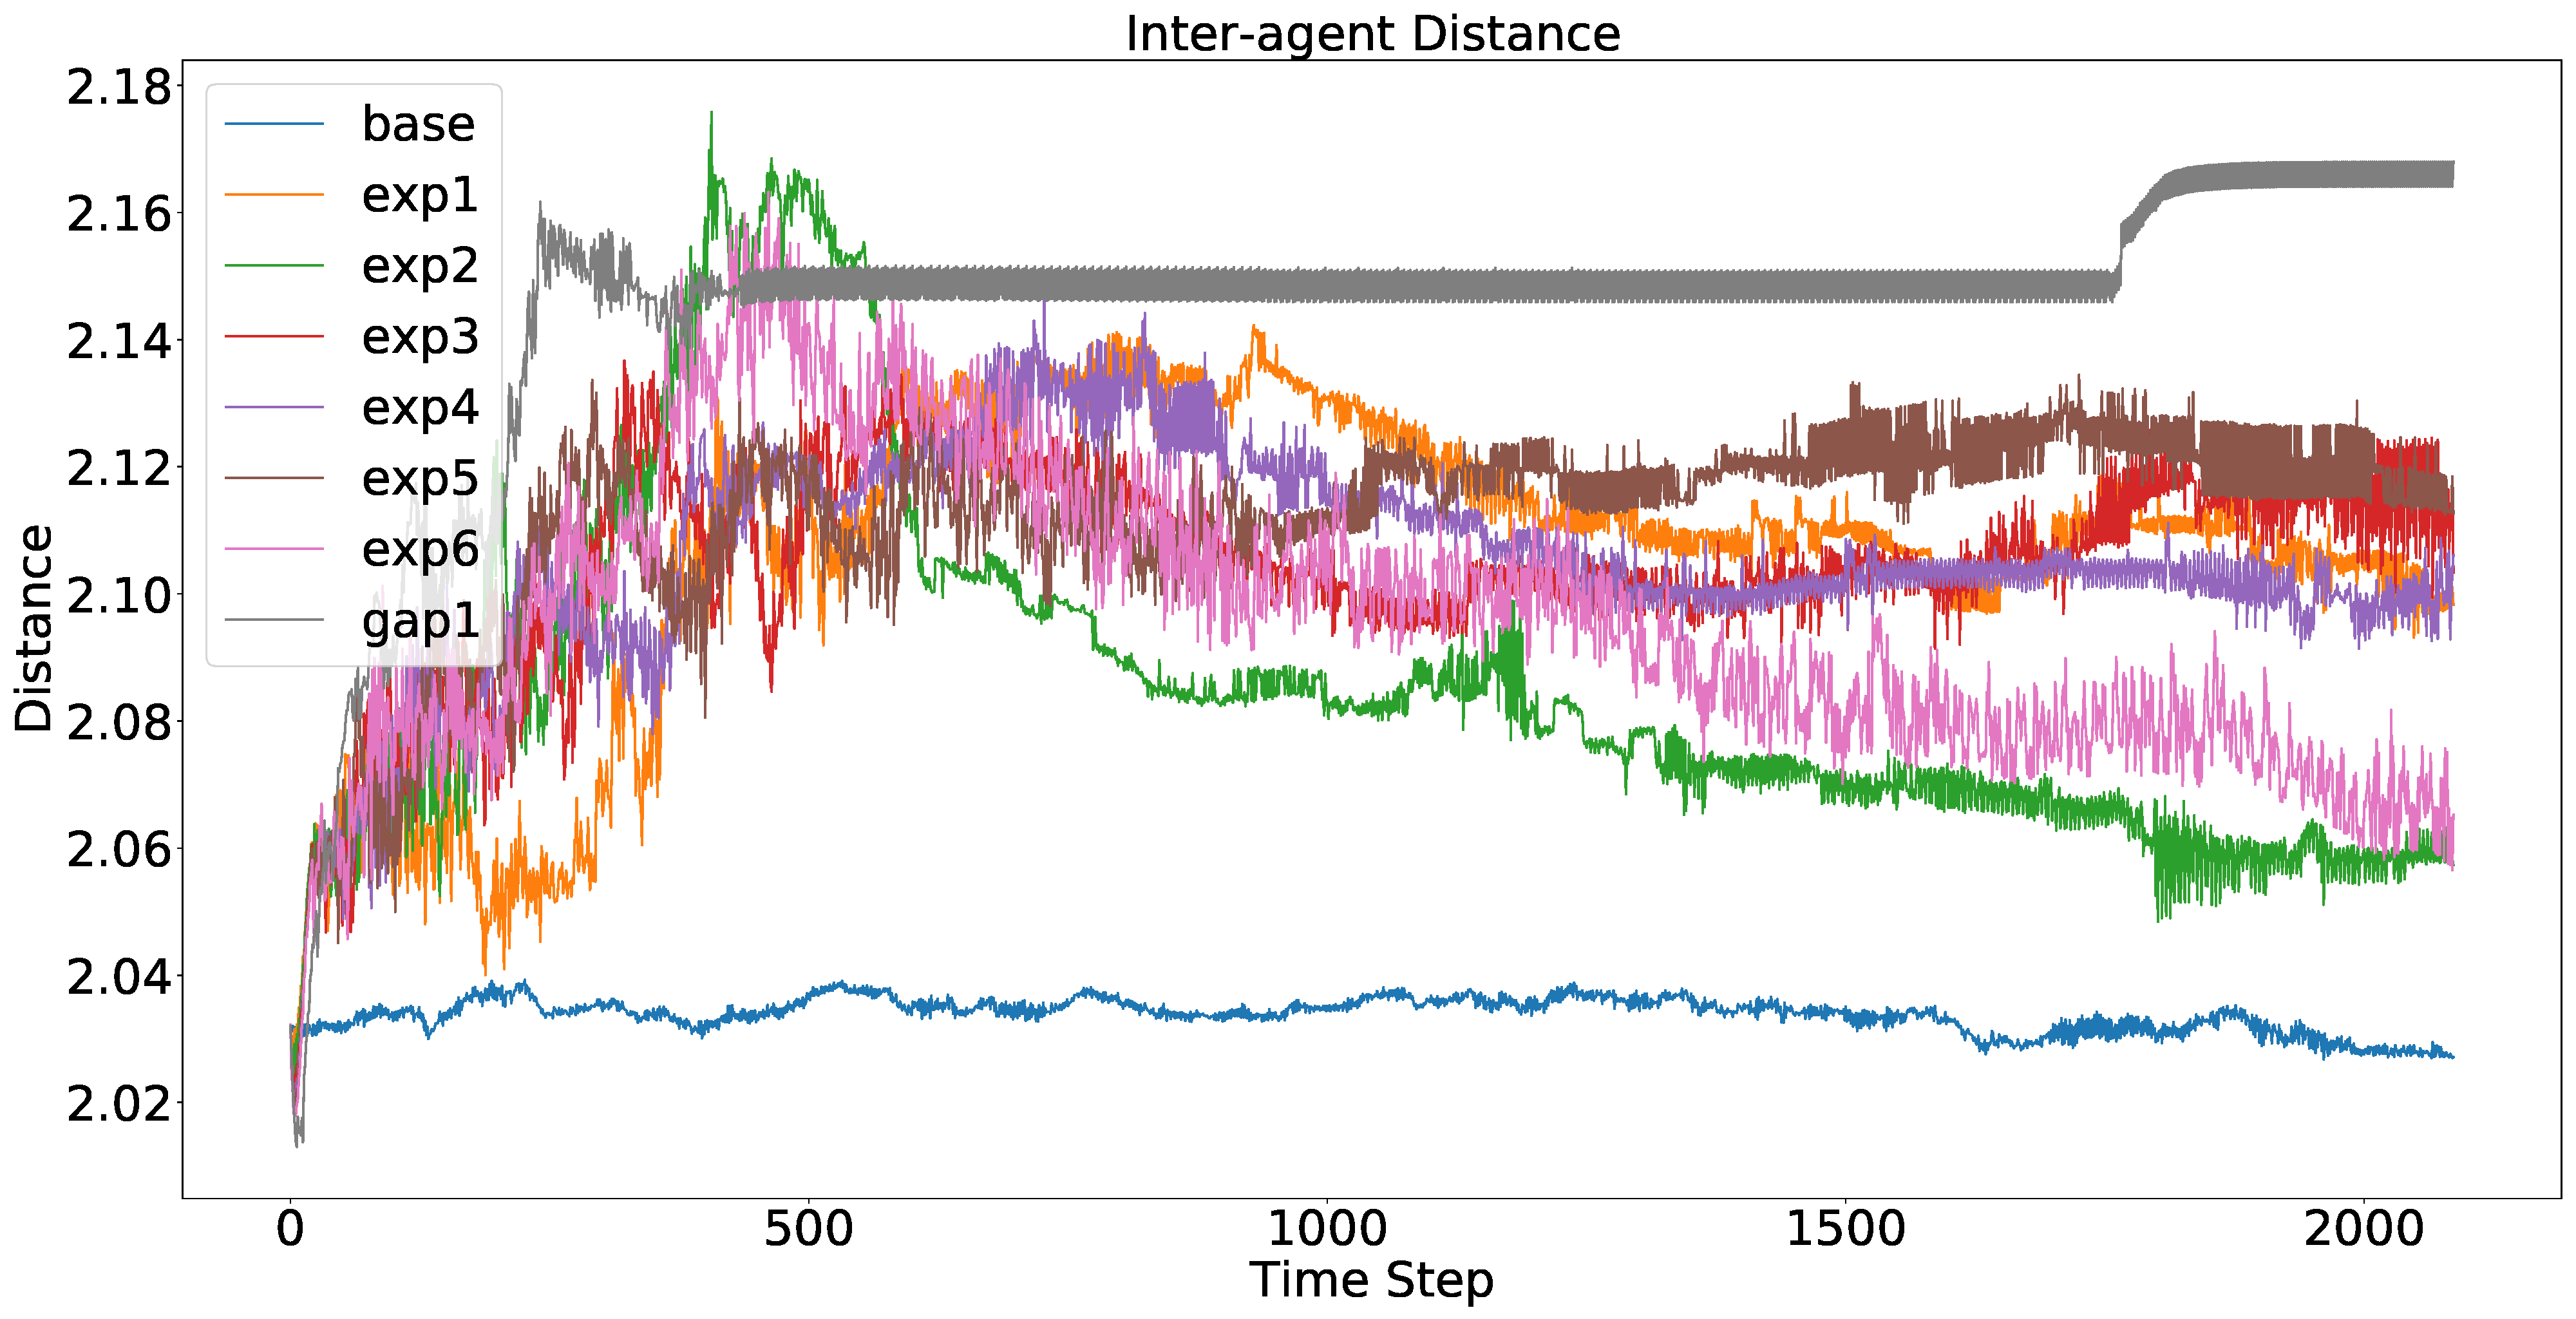
\includegraphics[width=8cm]{figures/DistanceMetric1}
	\end{center}
	\caption{Distance metric of baseline, gap reduction and perimeter compression. \label{fig:distanceMetric}}
\end{figure}

\begin{figure}[H]
	\begin{center}
		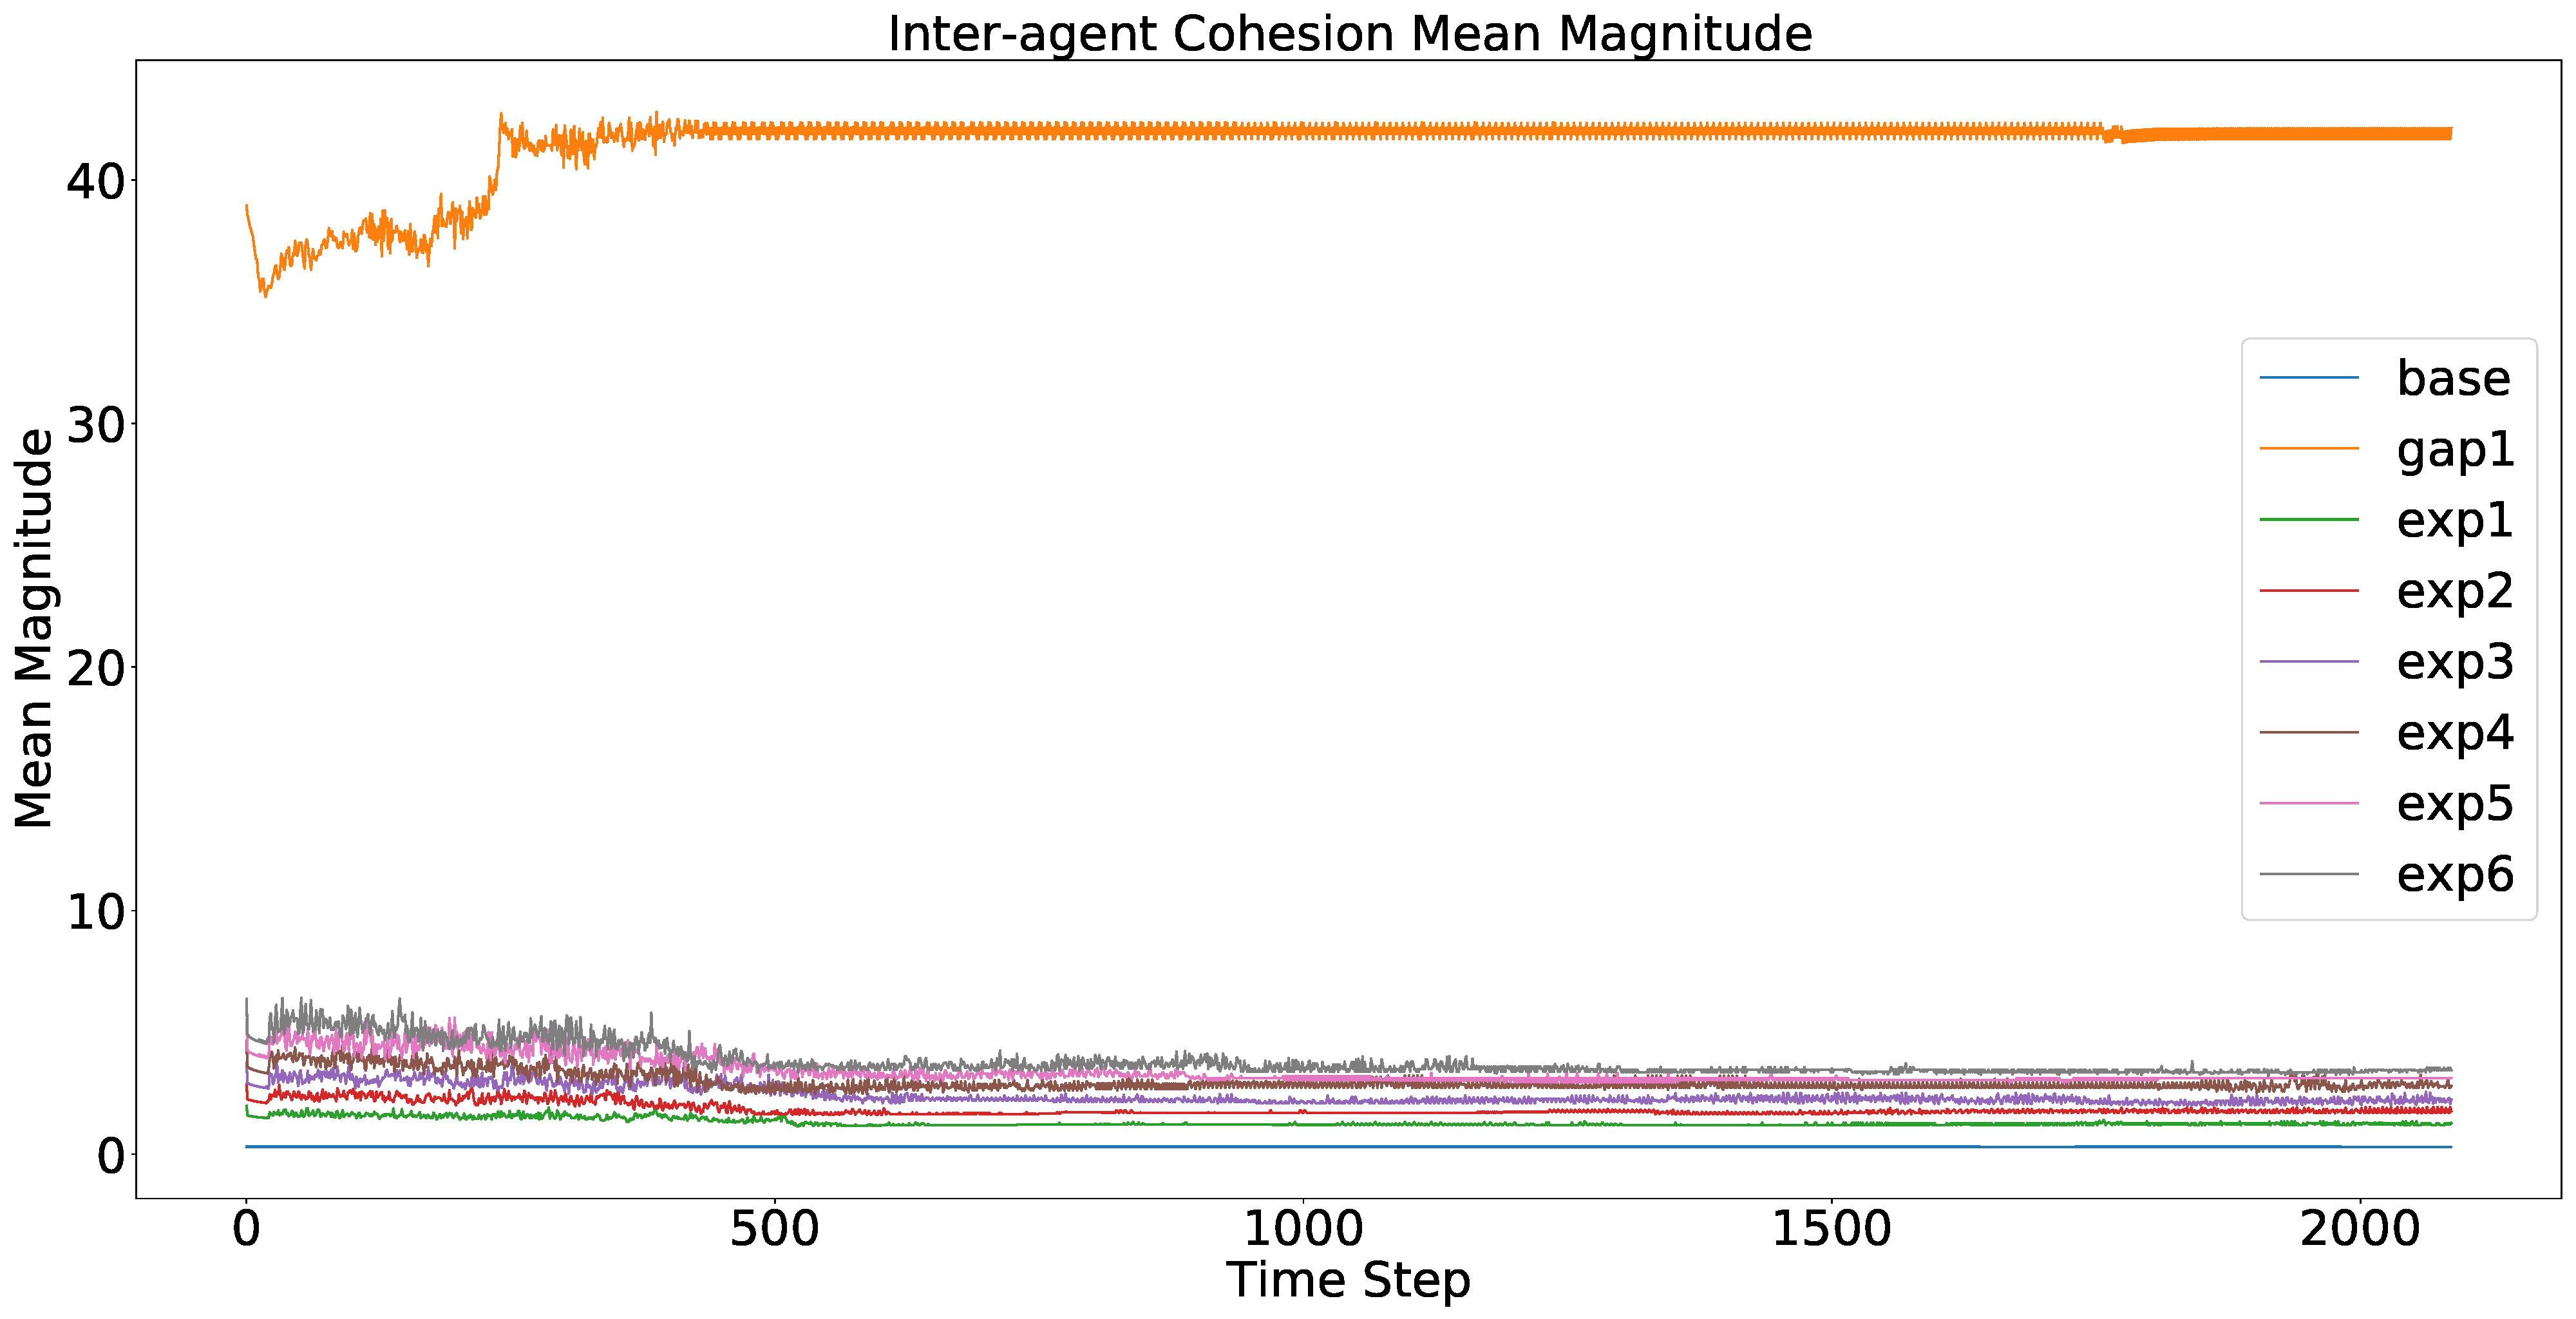
\includegraphics[width=8cm]{figures/InteragentCohesionMean}
	\end{center}
	\caption{Inter-agent Cohesion Mean. \label{fig:interagentCohesionMean}}
\end{figure}

\begin{figure}[H]
	\begin{center}
		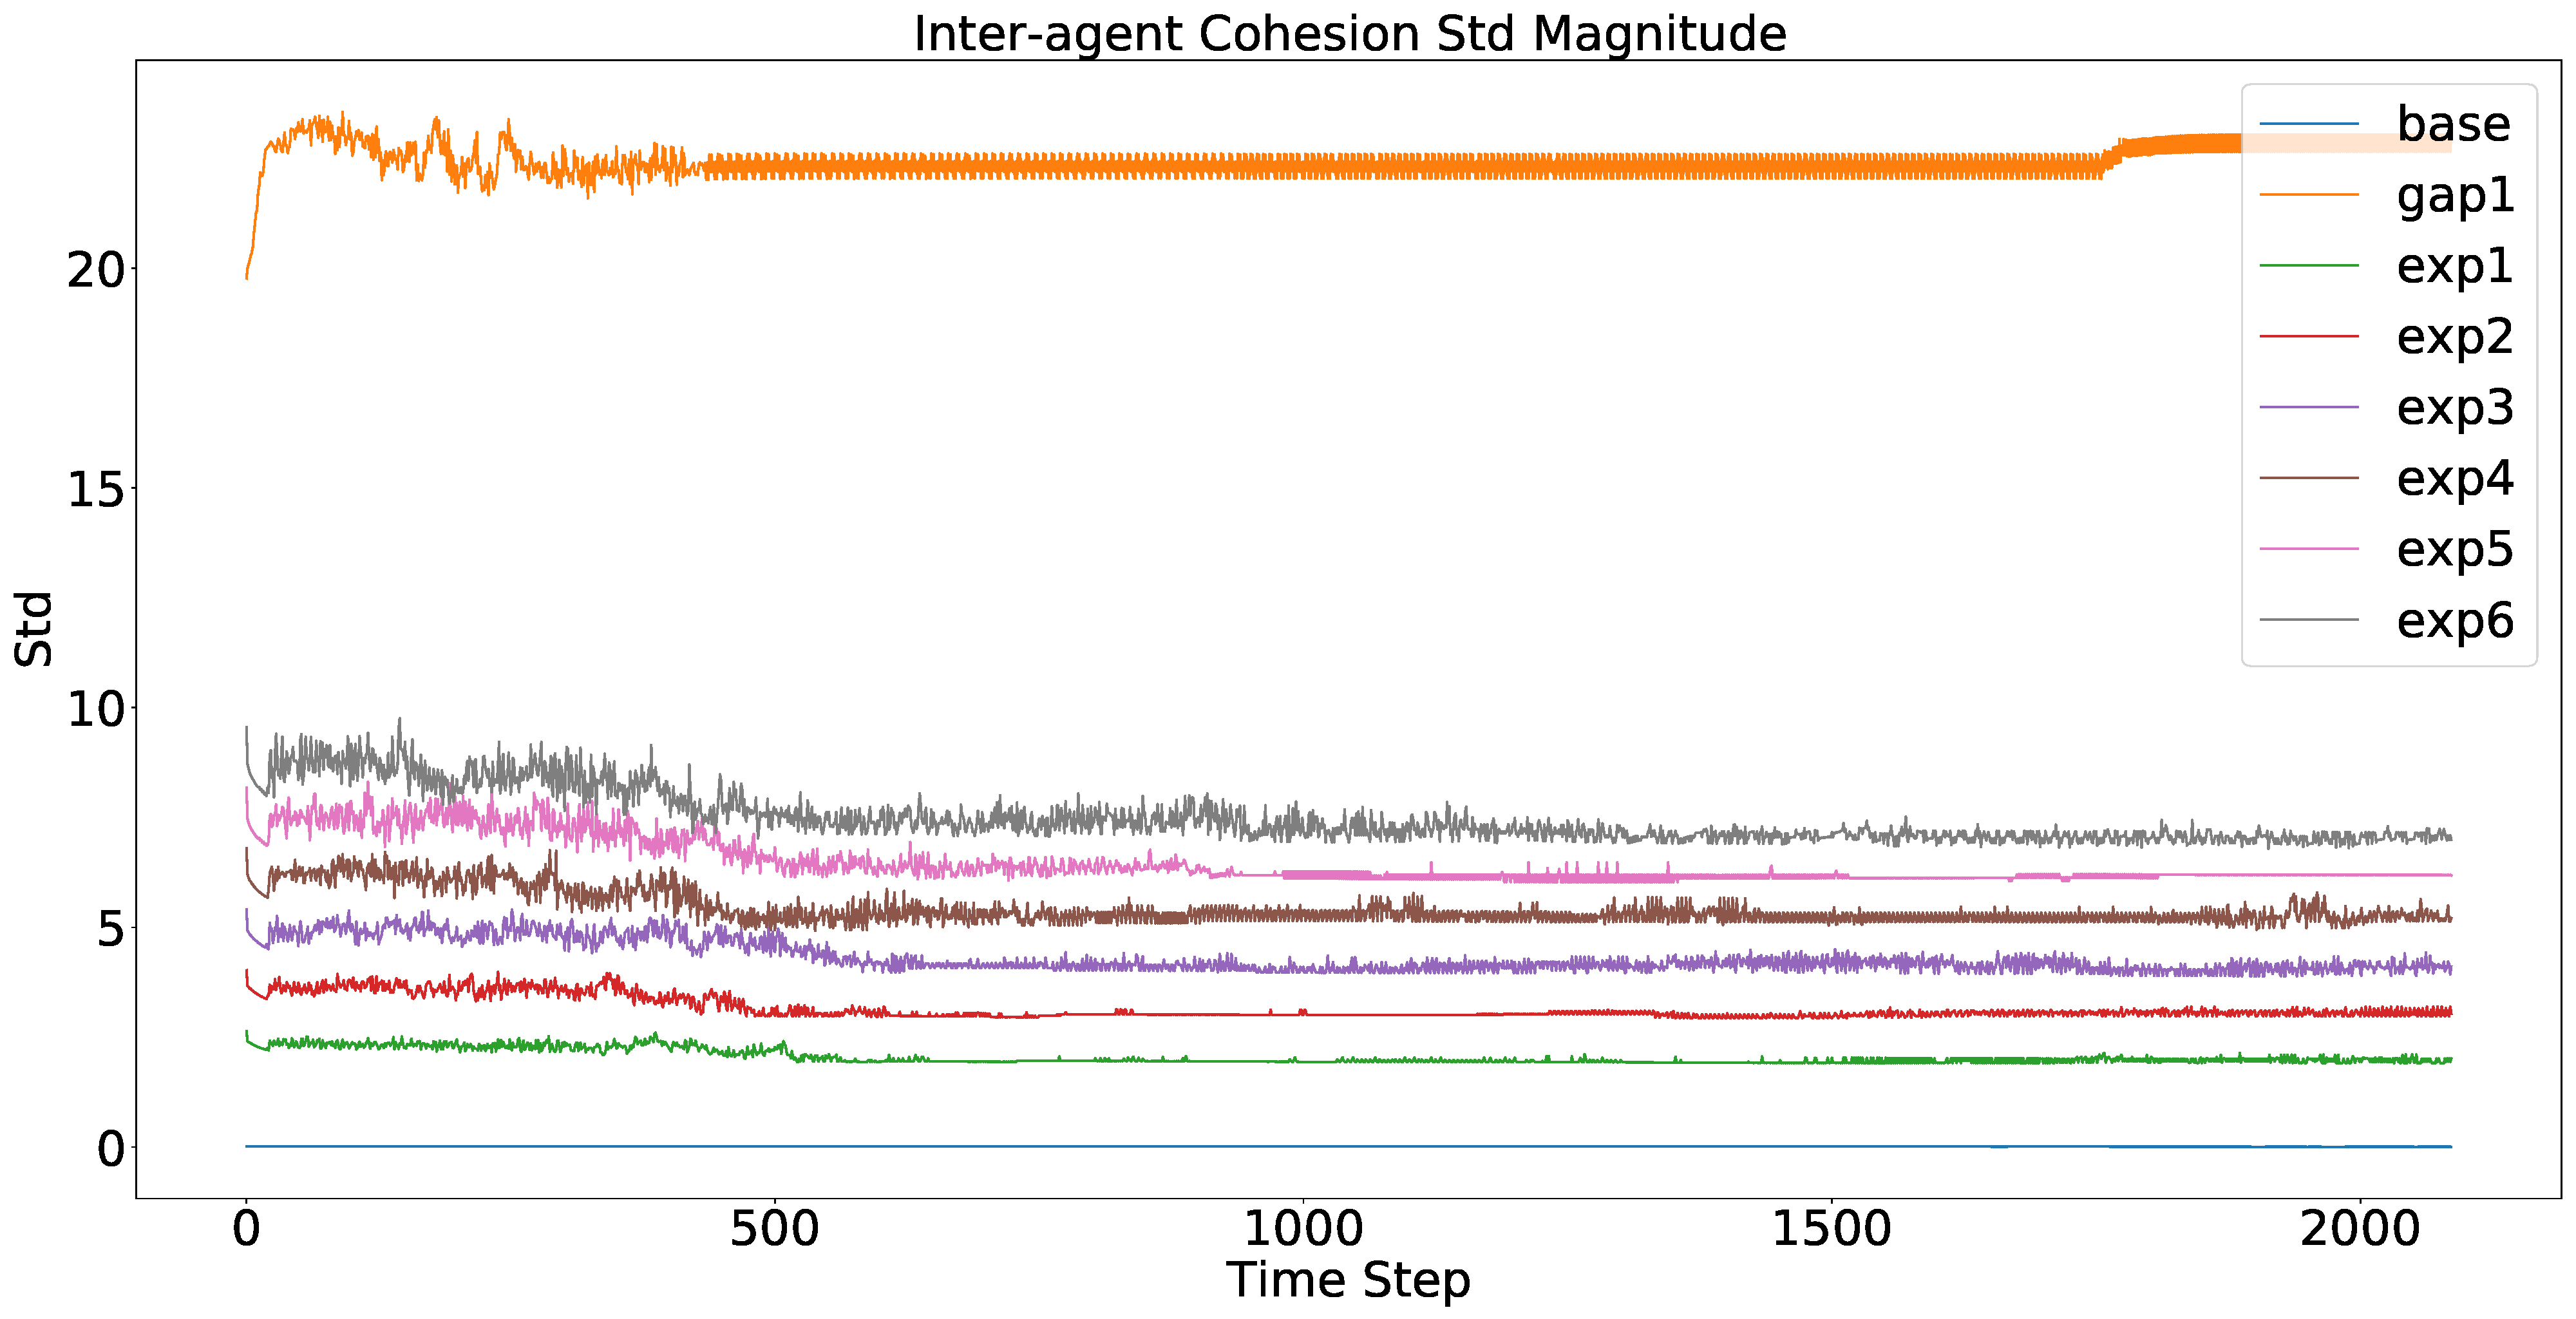
\includegraphics[width=8cm]{figures/InteragentCohesionStd}
	\end{center}
	\caption{Inter-agent Cohesion Std. \label{fig:interagentCohesionStd}}
\end{figure}

\begin{figure}[H]
	\begin{center}
		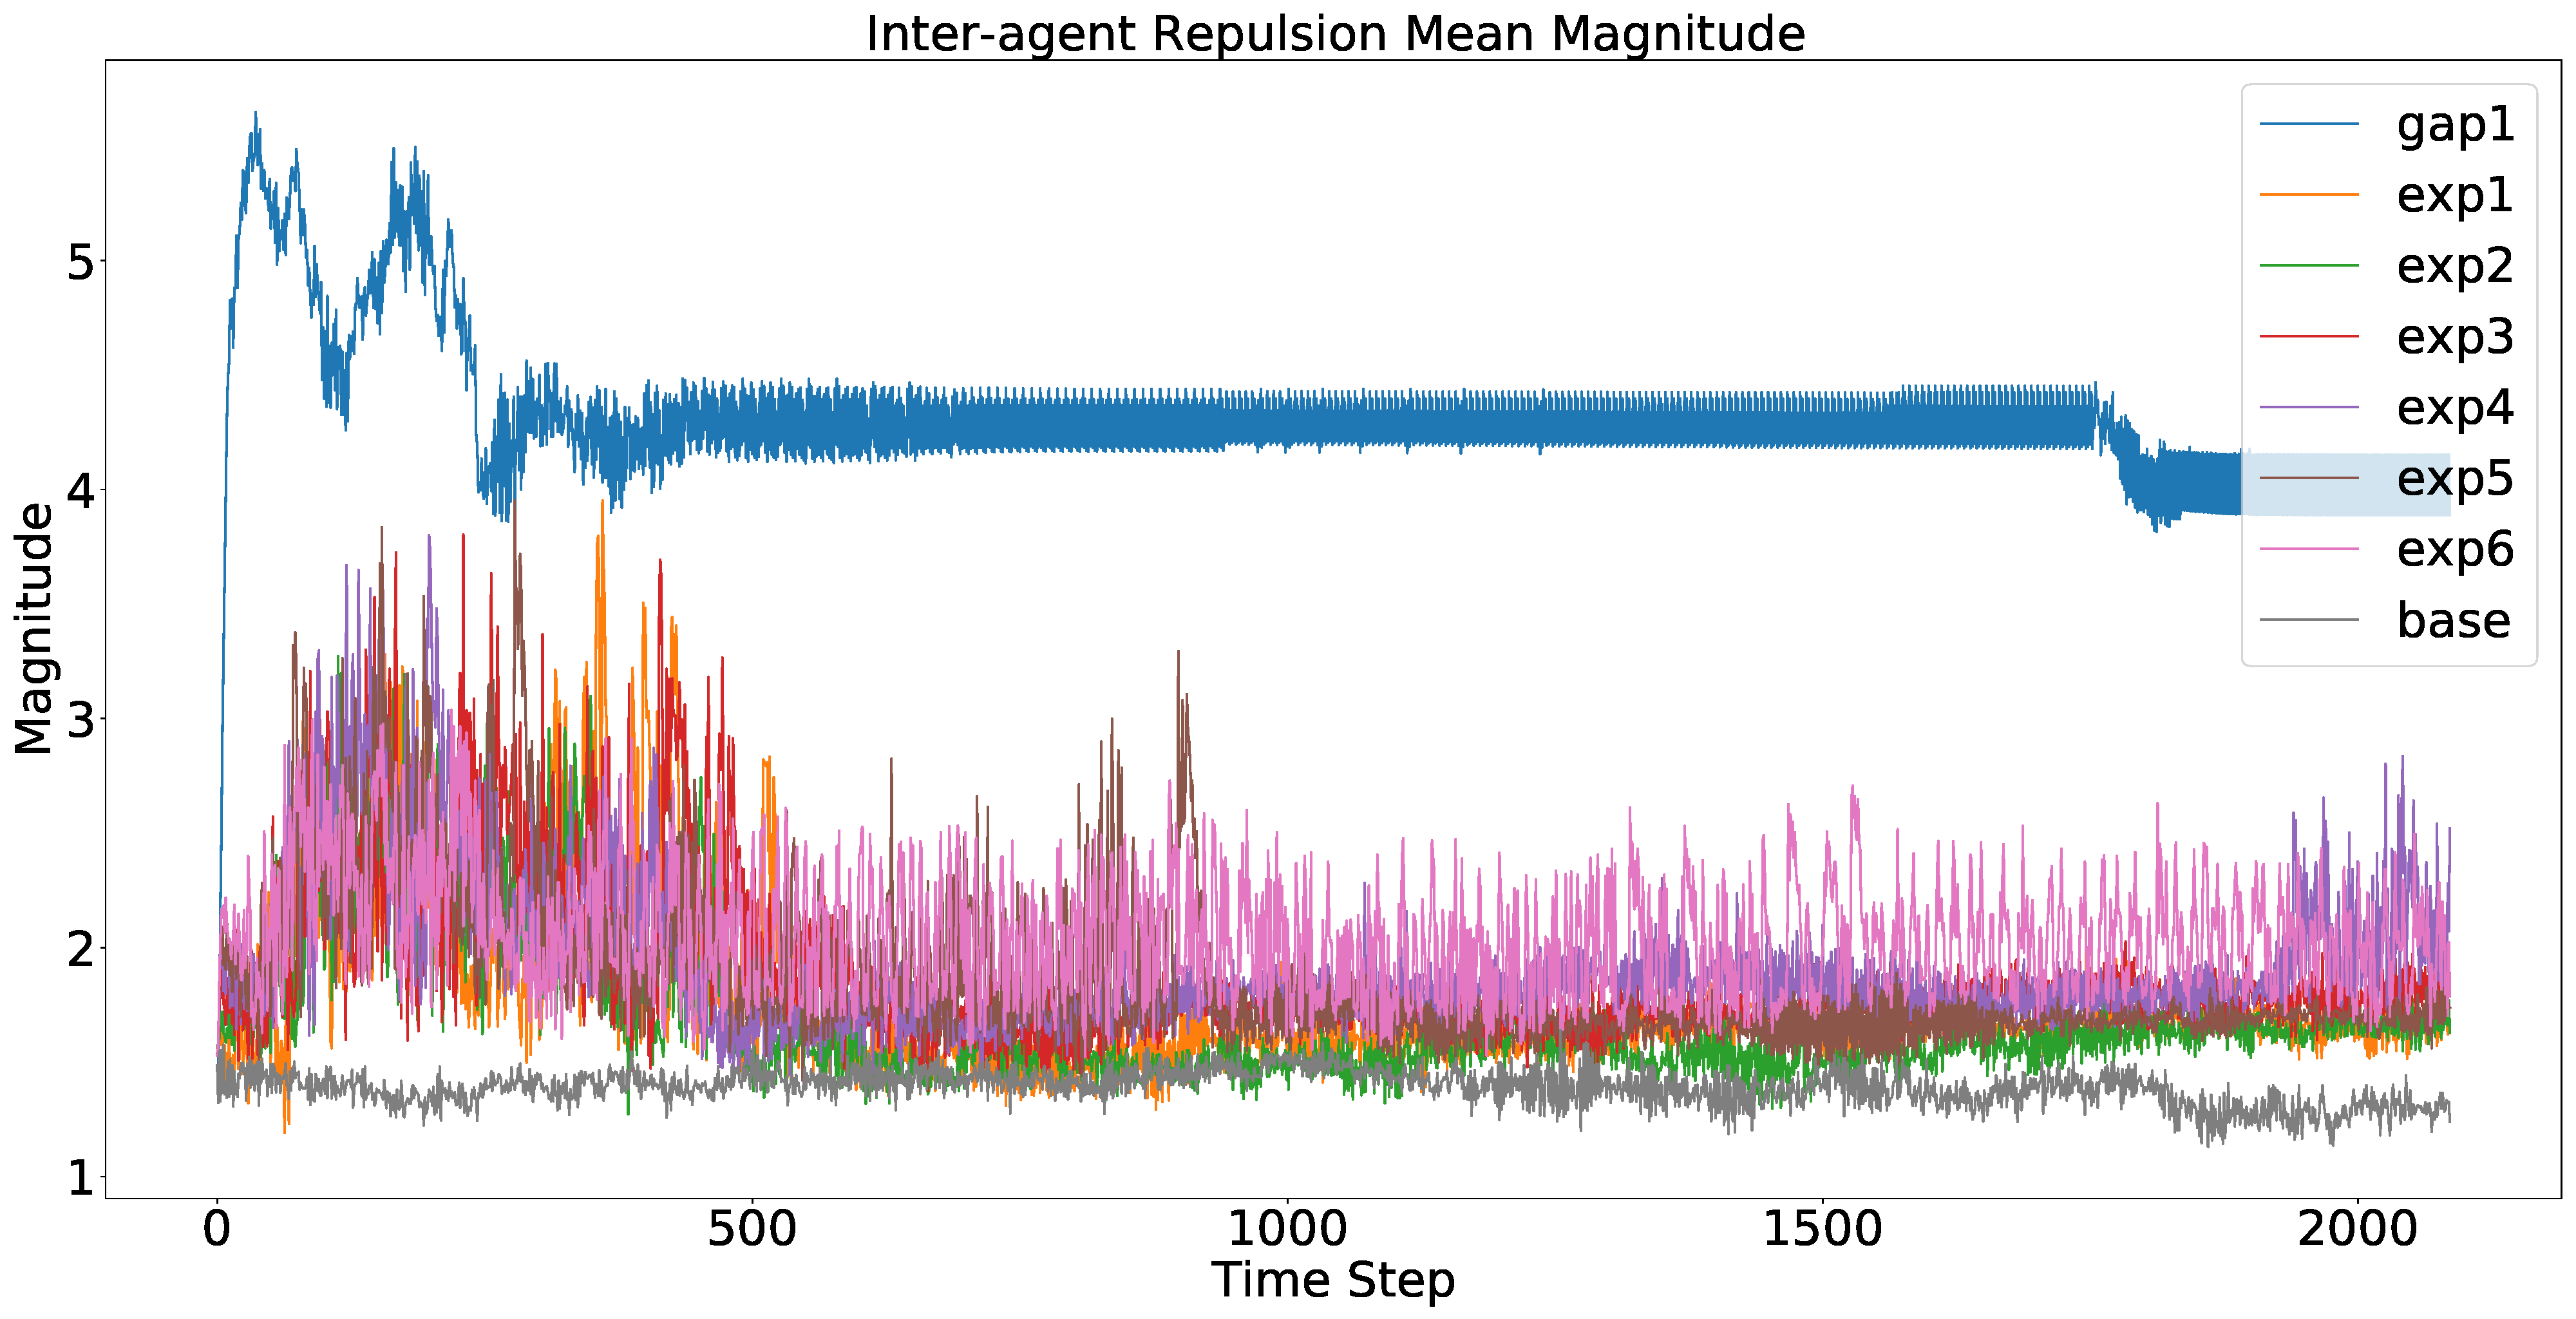
\includegraphics[width=8cm]{figures/InteragentRepulsionMean}
	\end{center}
	\caption{Inter-agent Repulsion Mean. \label{fig:interagentRepulsionMean}}
\end{figure}

\begin{figure}[H]
	\begin{center}
		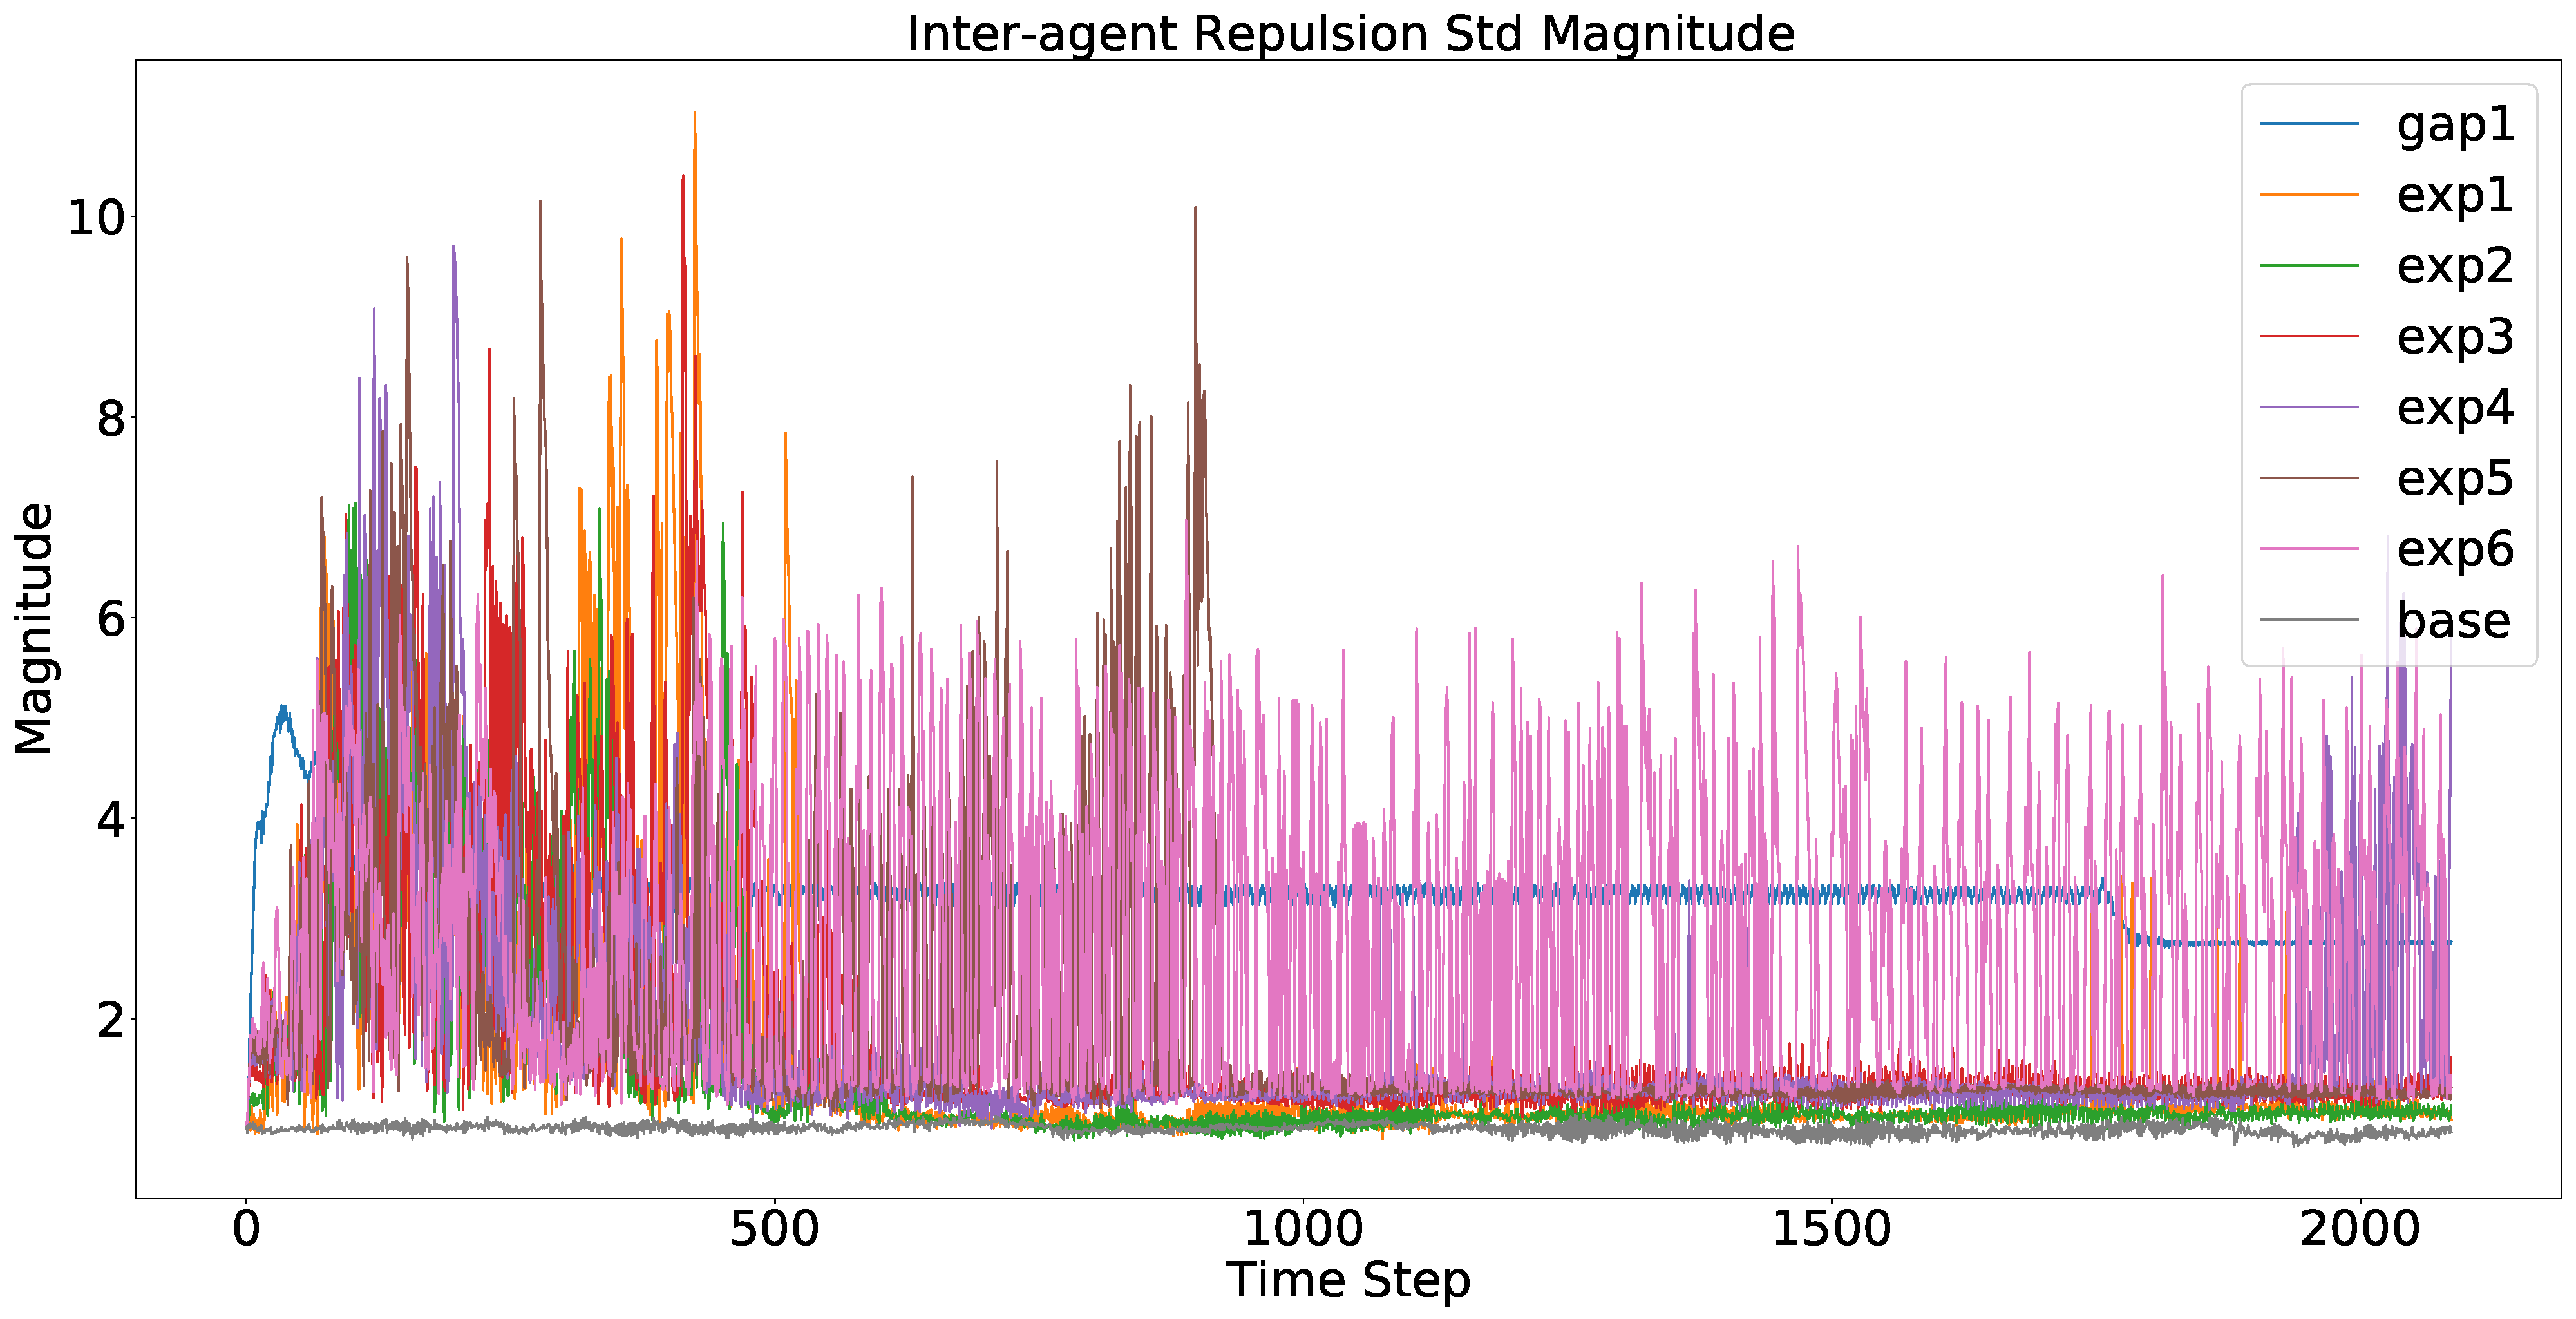
\includegraphics[width=8cm]{figures/InteragentRepulsionStd}
	\end{center}
	\caption{Inter-agent Repulsion Std. \label{fig:interagentRepulsionStd}}
\end{figure}


\begin{figure}[H]
	\begin{center}
		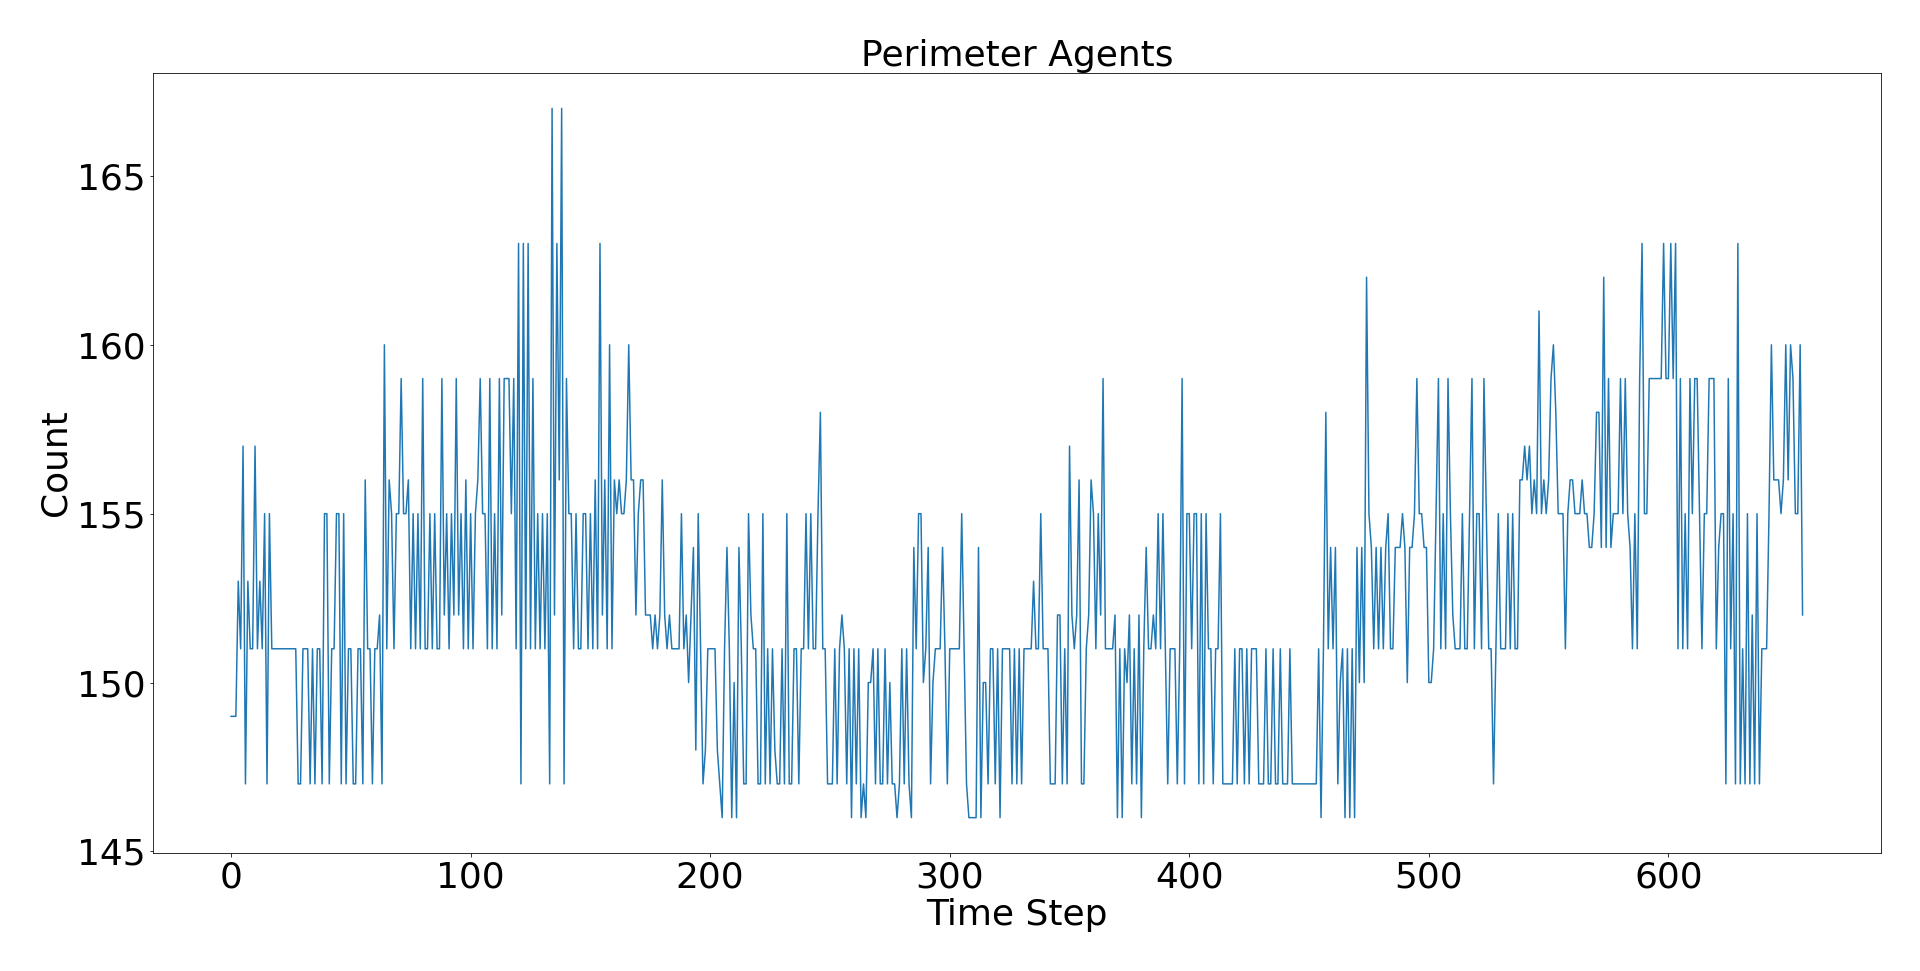
\includegraphics[width=8cm]{figures/baselineSwarmPerimeter}
	\end{center}
	\caption{Baseline swarm in stabilised configuration. \label{fig:baselineSwarmPerimeter}}
\end{figure}

\subsection{Gap compression}
\subsection{Perimeter compression}

Compression 1

\begin{figure}[H]
	\begin{center}
		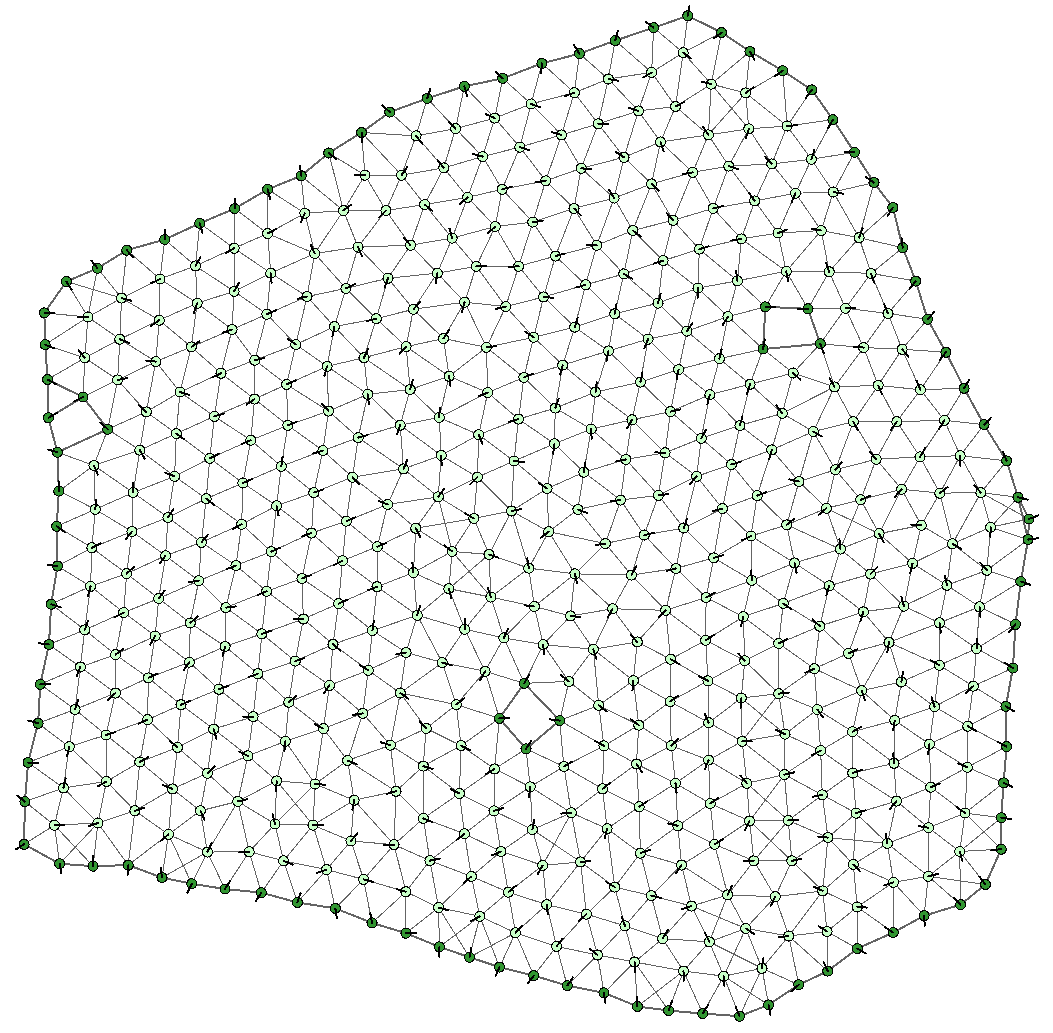
\includegraphics[width=5cm]{figures/baselineSwarm1}
	\end{center}
	\caption{Baseline swarm in with compression set 1 resultant configuration. \label{fig:baselineSwarm1}}
\end{figure}

\begin{figure}[H]
	\begin{center}
		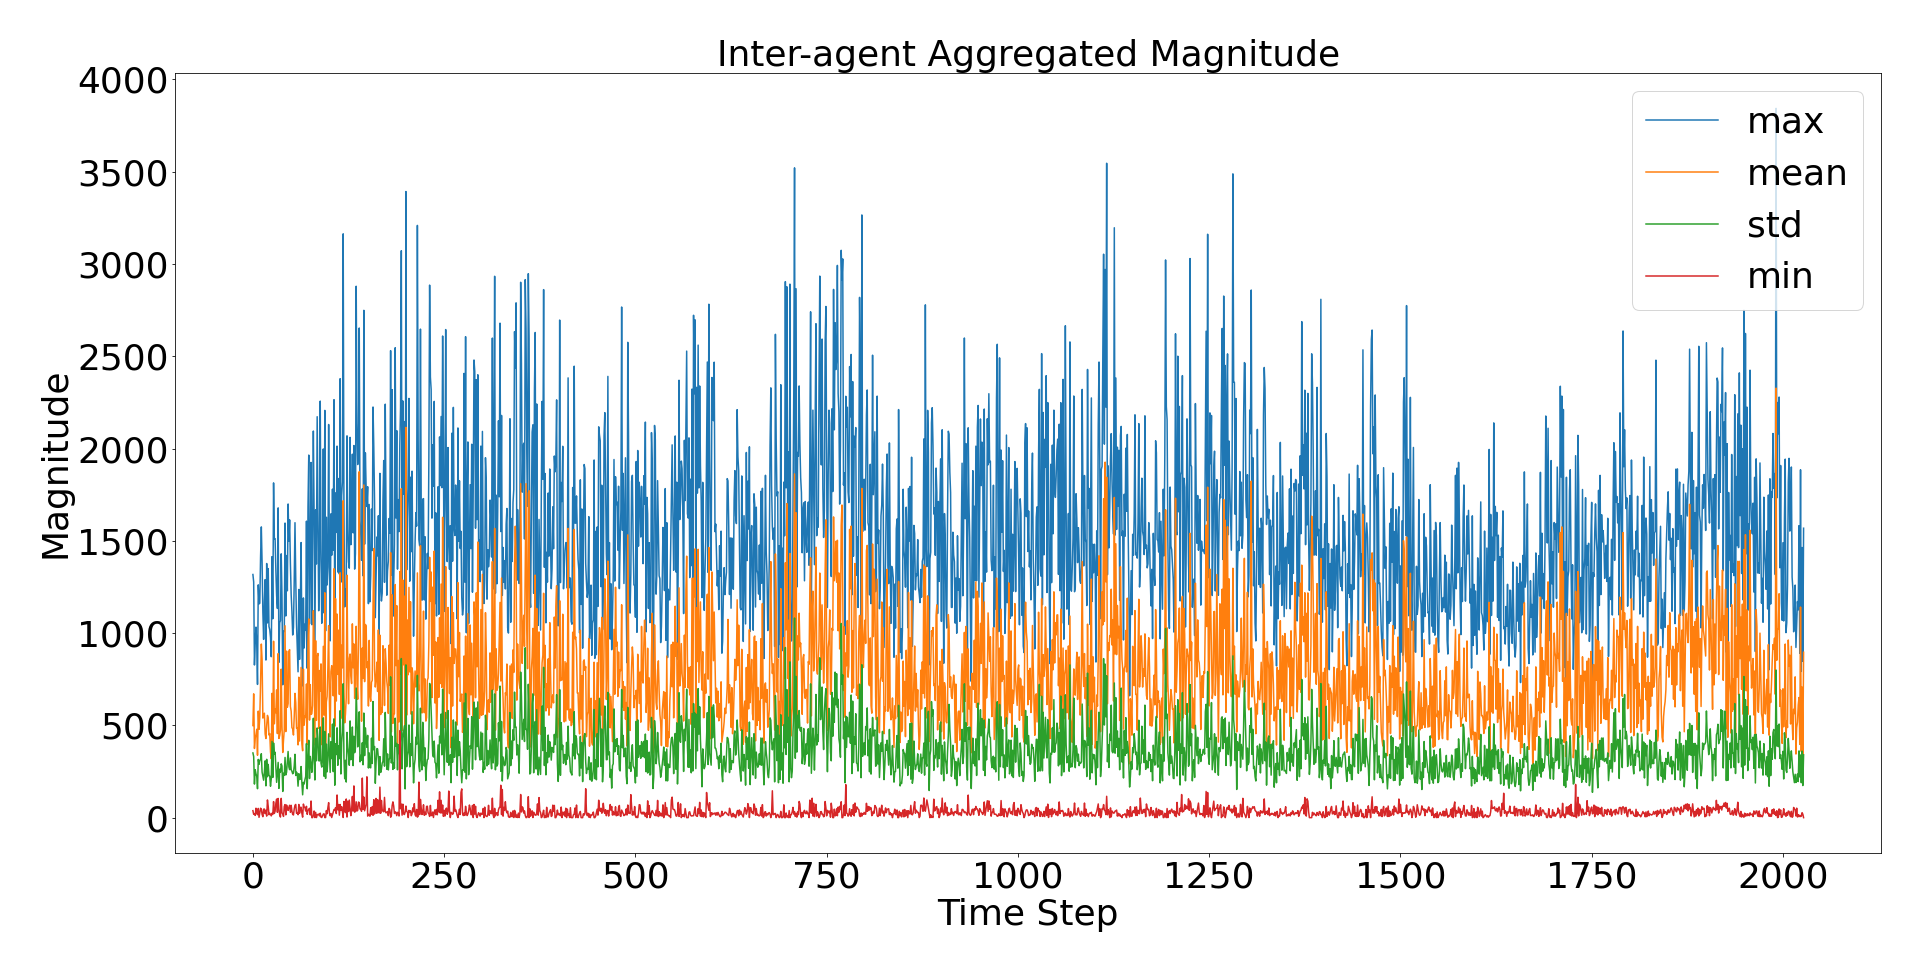
\includegraphics[width=8cm]{figures/baselineSwarmMagnitude1}
	\end{center}
	\caption{Baseline swarm in with compression set 1. \label{fig:baselineSwarmMagnitude1}}
\end{figure}

\begin{figure}[H]
	\begin{center}
		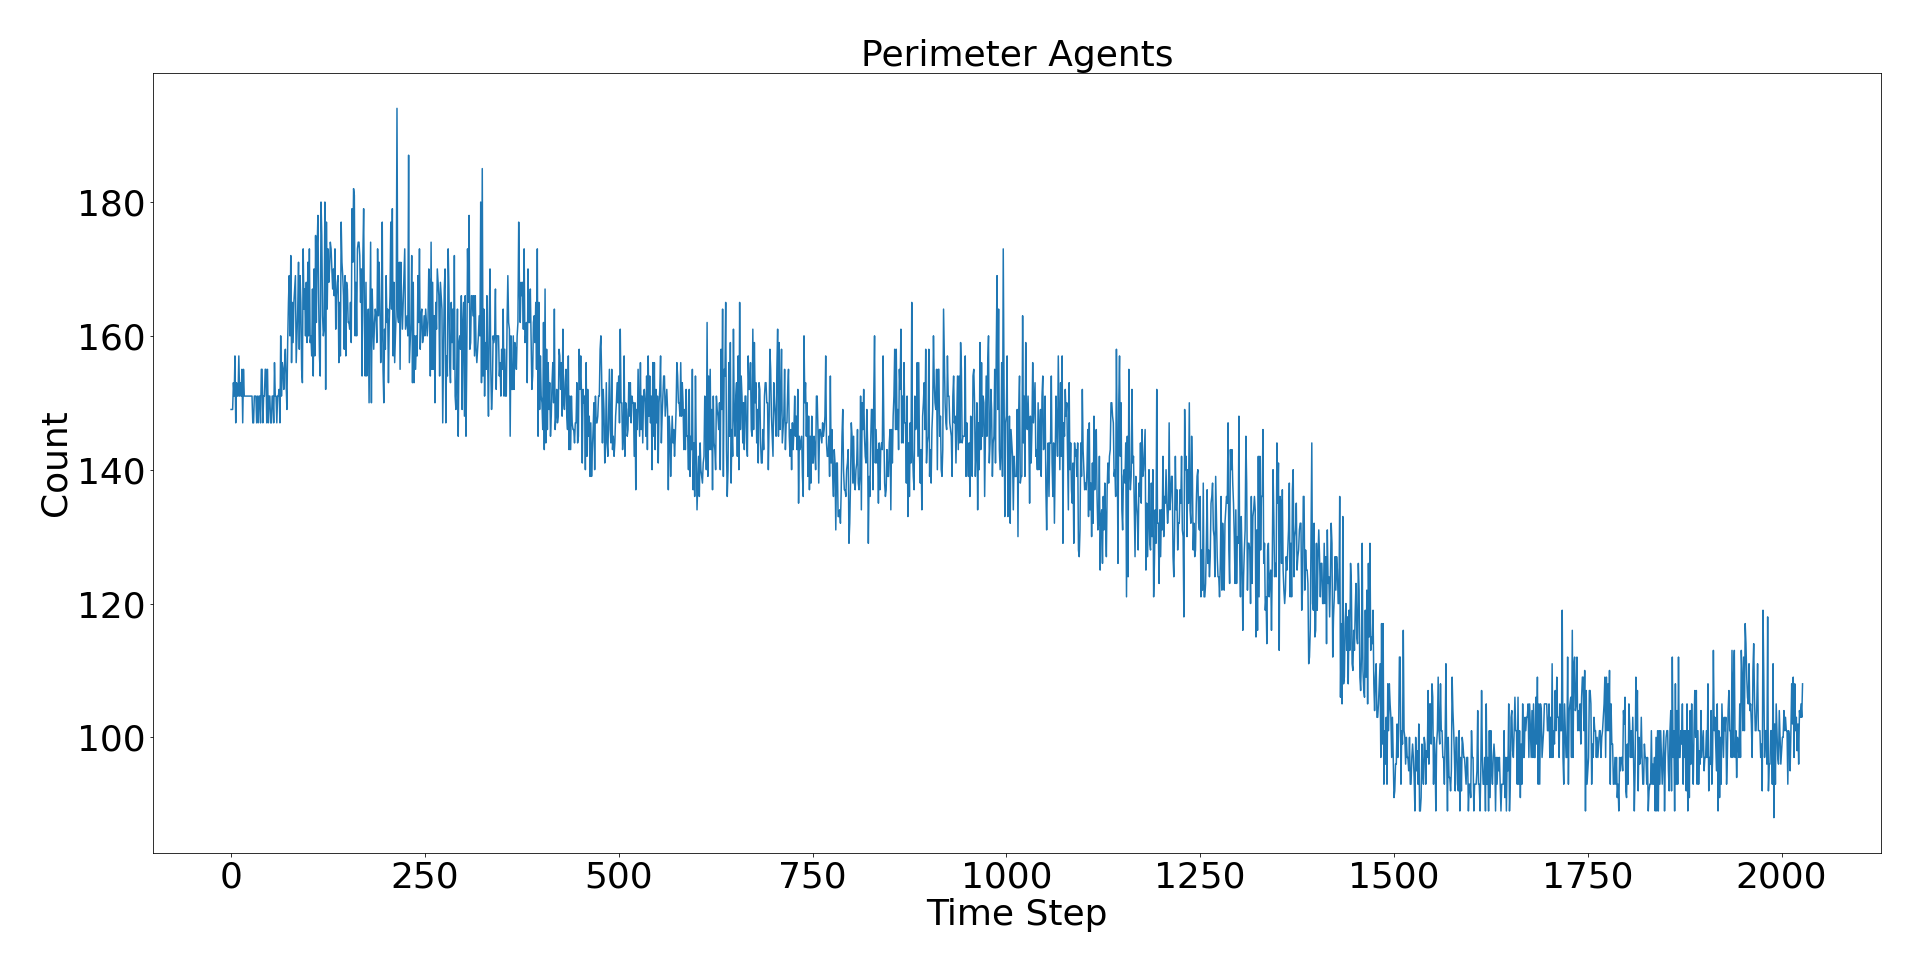
\includegraphics[width=8cm]{figures/baselineSwarmPerimeter1}
	\end{center}
	\caption{Baseline swarm in with compression set 1. \label{fig:baselineSwarmPerimeter1}}
\end{figure}

\subsection{Comparison}

\section{Conclusions}\label{conclusions}
From the initial simulations it is possible to show that the technique is able to successfully remove voids and surround an obstacle as shown in the video \href{https://youtu.be/3eY1vvq0JWo}{https://youtu.be/3eY1vvq0JWo}.

\section{Future Work}

\bibliographystyle{abbrv}
\bibliography{perimeter}

\end{document}